% Options for packages loaded elsewhere
\PassOptionsToPackage{unicode}{hyperref}
\PassOptionsToPackage{hyphens}{url}
\documentclass[
]{article}
\usepackage{xcolor}
\usepackage{amsmath,amssymb}
\setcounter{secnumdepth}{-\maxdimen} % remove section numbering
\usepackage{iftex}
\ifPDFTeX
  \usepackage[T1]{fontenc}
  \usepackage[utf8]{inputenc}
  \usepackage{textcomp} % provide euro and other symbols
\else % if luatex or xetex
  \usepackage{unicode-math} % this also loads fontspec
  \defaultfontfeatures{Scale=MatchLowercase}
  \defaultfontfeatures[\rmfamily]{Ligatures=TeX,Scale=1}
\fi
\usepackage{lmodern}
\ifPDFTeX\else
  % xetex/luatex font selection
\fi
% Use upquote if available, for straight quotes in verbatim environments
\IfFileExists{upquote.sty}{\usepackage{upquote}}{}
\IfFileExists{microtype.sty}{% use microtype if available
  \usepackage[]{microtype}
  \UseMicrotypeSet[protrusion]{basicmath} % disable protrusion for tt fonts
}{}
\makeatletter
\@ifundefined{KOMAClassName}{% if non-KOMA class
  \IfFileExists{parskip.sty}{%
    \usepackage{parskip}
  }{% else
    \setlength{\parindent}{0pt}
    \setlength{\parskip}{6pt plus 2pt minus 1pt}}
}{% if KOMA class
  \KOMAoptions{parskip=half}}
\makeatother
\usepackage{graphicx}
\makeatletter
\newsavebox\pandoc@box
\newcommand*\pandocbounded[1]{% scales image to fit in text height/width
  \sbox\pandoc@box{#1}%
  \Gscale@div\@tempa{\textheight}{\dimexpr\ht\pandoc@box+\dp\pandoc@box\relax}%
  \Gscale@div\@tempb{\linewidth}{\wd\pandoc@box}%
  \ifdim\@tempb\p@<\@tempa\p@\let\@tempa\@tempb\fi% select the smaller of both
  \ifdim\@tempa\p@<\p@\scalebox{\@tempa}{\usebox\pandoc@box}%
  \else\usebox{\pandoc@box}%
  \fi%
}
% Set default figure placement to htbp
\def\fps@figure{htbp}
\makeatother
\setlength{\emergencystretch}{3em} % prevent overfull lines
\providecommand{\tightlist}{%
  \setlength{\itemsep}{0pt}\setlength{\parskip}{0pt}}
\usepackage{bookmark}
\IfFileExists{xurl.sty}{\usepackage{xurl}}{} % add URL line breaks if available
\urlstyle{same}
\hypersetup{
  hidelinks,
  pdfcreator={LaTeX via pandoc}}

\author{}
\date{}

\begin{document}

{Cloud computing}

{}

\section{\texorpdfstring{{Storia}}{Storia}}\label{h.jlzz23tflqtu}

{Idea nata nel `61 da John McCarthy, che consisteva nel fornire capacità
di calcolo come un utility, ma mancavano le tecnologie. Negli anni 70
c'è la prima apparizione della virtualizzazione, dove viene diviso un
server in chunk con proprie risorse e S.O. verrà chiamato macchina
virtuale.}

{Negli anni 90 iniziano le distribuzioni di software via internet ma per
farlo servono grossi datacenter, all'inizio in housing con molte
problematiche relative alla scalabilità, infatti se gli utenti crescono
deve crescere la potenza ma se scendono la potenza superflua è una spesa
inutile (costi di server, manutenzione e montaggio).}

{Per questo Salesforce inizia a fornire un Software as a Service (SaaS),
ovvero un\textquotesingle applicazione utilizzabile da chiunque, via
internet, che risiede nei loro server e gestibile da remoto dall'azienda
che non si accorge di lavorare in un server condiviso con tanti altri
utenti.}

{}

{Dal 2000 le principali aziende iniziano a creare datacenter per il
globo per fornire servizi con latenze basse, nel 2006 Amazon lancia AWS
dove noleggia lo spazio dei propri datacenter non utilizzato, seguito
successivamente da Google e
Microsoft.}{\pandocbounded{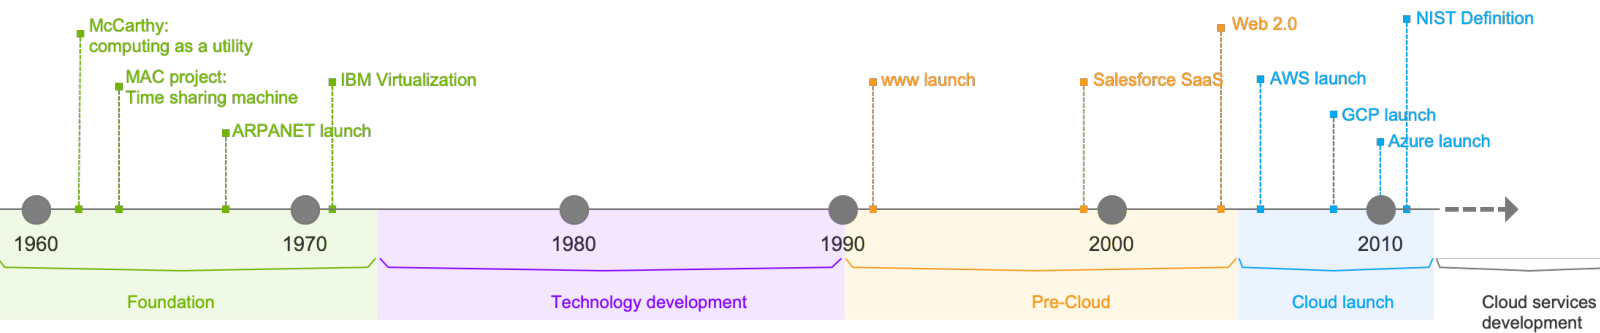
\includegraphics[keepaspectratio]{images/image26.png}}}

{}

{}

{}

{}

{}

{}

{}

{}

{Definizione (formale):}

{}

{Cloud computing is a model for enabling ubiquitous, convenient,
ondemand network access to a shared pool of configurable computing
resources (e.g., networks, servers, storage, applications, and services)
that can be rapidly provisioned and released with minimal management
effort or service provider interaction. This cloud model is composed of
five essential characteristics, three service models, and four
deployment models}

{}

\section{\texorpdfstring{{Caratteristiche}}{Caratteristiche}}\label{h.b44wxi9l58r8}

{Secondo il NIST il cloud prevede 5 (almeno) caratteristiche:}

\begin{enumerate}
\tightlist
\item
  {On-demand, self-service}{: risorse attive solo quando servono in
  maniera automatica;}
\item
  {Broad network access}{: si può accedere via internet con client
  eterogenei;}
\item
  {Resource pooling}{: risorse in comune fra tutti i clienti
  (multi-tenant) e (ri)assegnate in base alle richieste dei singoli. I
  client non sanno dove sono collocate le risorse, possono scegliere al
  massimo la posizione (approssimata) del datacenter utilizzato;}
\item
  {Rapid elasticity}{: diminuzione e aumento delle risorse in maniera
  rapida, elastica e/o automatico}
\item
  {Measured service}{: chi fornisce il servizio monitora e ottimizza
  l'uso delle risorse.}
\end{enumerate}

{}

\section{\texorpdfstring{{Successo}}{Successo}}\label{h.ihbpafyt88tx}

{I fattori sono:}

\begin{itemize}
\tightlist
\item
  {modello di costo}{: paghi solo quello che richiedi in base al tempo
  di utilizzo (PAYG) con costi bassi grazie ad economie di scala (+
  clienti - costi) e senza investimenti iniziali (CapEx - Capital
  Expenditure).}
\item
  {scalabilità}{: puoi aumentare o diminuire risorse quando vuoi senza
  problemi visto che i data center e tutto ciò al suo interno è gestito
  dal provider;}
\item
  {disponibilità}{: accedi e usi quando vuoi e dove vuoi.}
\item
  {affidabilità}{: il cloud funzionerà sempre e senza errori;}
\item
  {durabilità}{: i tuoi dati saranno sempre al sicuro da perdite o
  corruzione da errori da fuori e da dentro;}
\item
  {sicurezza}{: protezione da accessi non autorizzati.}
\end{itemize}

{}

\section{\texorpdfstring{{Cloud Service
Models}}{Cloud Service Models}}\label{h.lv71tcb9i931}

{Il provider può fornire le proprie risorse su livelli diversi per
questo nascono i modelli di servizio.}

{Le risorse messe a disposizione sono sempre le stesse ma da modello a
modello cambia cosa gestisci tu e cosa gestisce il provider:}

{\pandocbounded{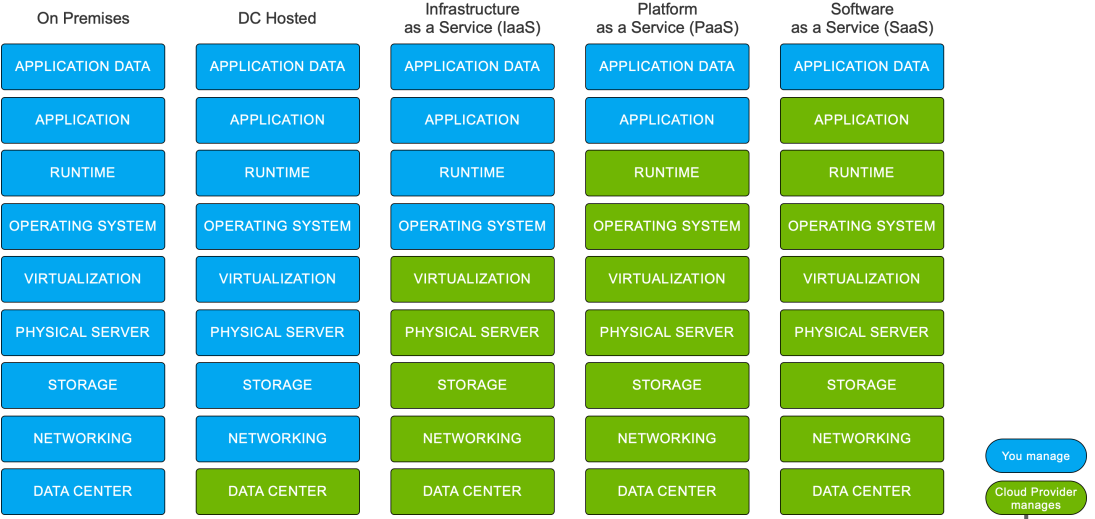
\includegraphics[keepaspectratio]{images/image31.png}}}

{}

{Nella parte verde (quella gestita dal provider) qualunque problema o
servizio è gestito senza che il cliente se ne debba preoccupare, al
contrario la parte blu è di sua responsabilità e quindi ogni problema
riscontrato non viene gestito dal provider. }

{}

{Questo modello dove ognuno è responsabile della propria parte di stack
è detta }{Shared responsibility model}{.}

{}

{I vari servizi sono:}

{}

\subsection{\texorpdfstring{{IaaS - Infrastructure as a
Service}}{IaaS - Infrastructure as a Service}}\label{h.j4fus0gjci28}

{Il provider gestisce tutto ciò a basso livello come la VM, lo storage
(virtuale) e il networking. Il cliente può decidere il S.O. e scaricare
qualsiasi software nella VM.}

{}

{Vengono usate vCPU cioè singole unità di elaborazione:}

{\pandocbounded{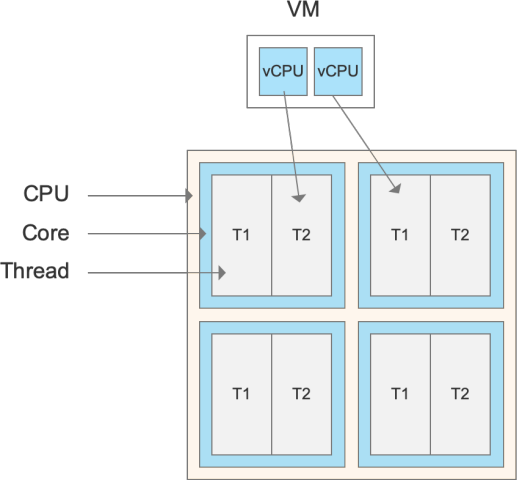
\includegraphics[keepaspectratio]{images/image55.png}}}

{Il disco invece è astratto in storage pools, }{combinazione di
tecnologie diverse}{~utilizzate come un'unica entità, permettendo
l'aggiunta o la rimozione spazio in maniera arbitraria.}

{}

{Per isolare logicamente a livello di rete le VM si usano reti virtuali
}{creare}{~su quella fisica; questo grazie a protocolli particolari che
permettono di creare connessioni virtuali tra nodi virtuali, mappando il
tutto sulla rete fisica }{(Overlay Network)}{.}

{\pandocbounded{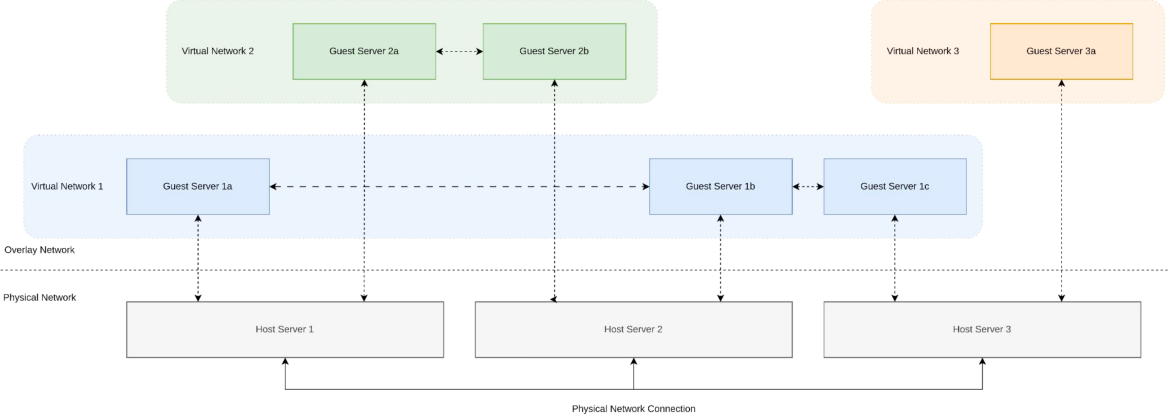
\includegraphics[keepaspectratio]{images/image59.png}}}

\subsubsection{\texorpdfstring{{Google Compute
Engine}}{Google Compute Engine}}\label{h.xzhpr27l2jm5}

{Soluzione IaaS di GCP, creazione/gestione/configurazione e connessione
di VM (istanze) con fatturazione al minuto.}

{}

{L'istanza è configurabile nei seguenti aspetti:}

{\pandocbounded{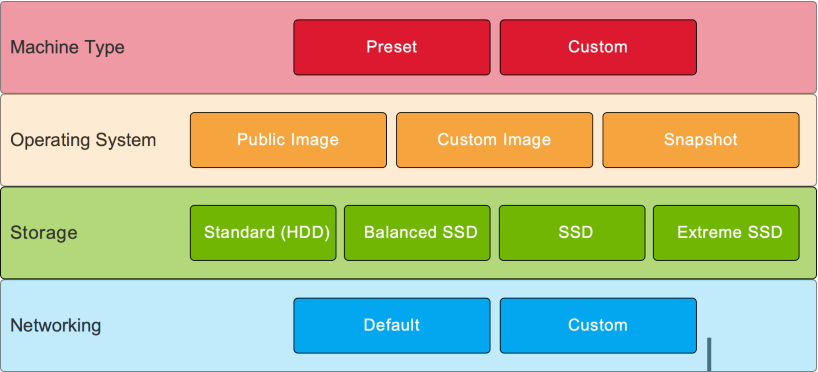
\includegraphics[keepaspectratio]{images/image37.png}}}

{}

\begin{itemize}
\tightlist
\item
  {Machine type}{: è possibile scegliere una tipologia divise in Series
  (determina la }{qtà}{~min/max di }{vCPU}{~e RAM).}
\end{itemize}

{Le serie possono essere:}

\begin{itemize}
\tightlist
\item
  {Preset}{: numero di }{vCPU}{~e RAM già deciso con il nome in questo
  formato:}
\end{itemize}

{\pandocbounded{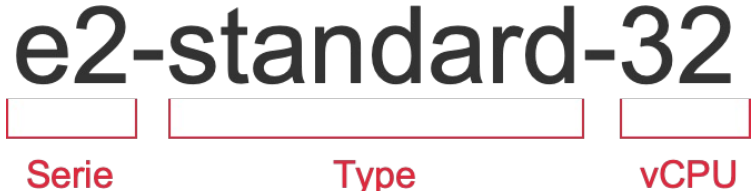
\includegraphics[keepaspectratio]{images/image33.png}}}

\begin{itemize}
\tightlist
\item
  {Custom}{: numero di }{vCPU}{~e RAM da decidere}
\end{itemize}

{}

\begin{itemize}
\tightlist
\item
  {Operating system}{: l'immagine per caricare il SO è scelto fra i
  seguenti modi:}
\end{itemize}

\begin{itemize}
\tightlist
\item
  {Public Images}{: Selezionato da un elenco predefinito di SO.}
\item
  {Custom Image}{: Selezionando un\textquotesingle immagine disco creata
  precedentemente, anche non in GCP.}
\item
  {Snapshot}{: Selezionando lo snapshot di un PD creato in precedenza}
\end{itemize}

{}

{L'images è una copia completa del disco dell'istanza utile per riusare
le istanze ma non supporta il disaster recovery; lo snapshot è una copia
del contenuto di un singolo Persistent Disk quindi perfetto per il
backup (supporto alla copia differenziale, cioè save dei soli dati
modificati rispetto allo snapshot prima).}

{}

\begin{itemize}
\tightlist
\item
  {Storage}{: l'istanza chiede almeno un disco con possibilità di
  inserirne altri successivamente.}
\end{itemize}

{I dischi che vengono collegati all\textquotesingle istanza sono detti
}{Persistent}{~Disk (PD), in quanto possono sopravvivere alla
cancellazione della VM e sono }{Standard}{, }{Balanced SSD}{, }{SSD }{o
}{Extreme SSD}{.}

{}

\begin{itemize}
\tightlist
\item
  {N}{etworking}{: ogni istanza è collegata ad una }{VPC}{~(Virtual
  Private Cloud) con di default un indirizzo pubblico per essere
  accessibile da internet.}
\end{itemize}

{}

{Esistono altri tipi di istanze dette }{spot }{o }{preemptible}{, che
possono essere interrotte quando vuoi e fortemente scontate, ma non
sempre disponibili e non coperte da SLA (Service Level Agreements).}

{}

{}

{}

{}

{Ogni istanza ha un proprio lifecycle dove può rientrare in alcuni di
questi stati:}

{\pandocbounded{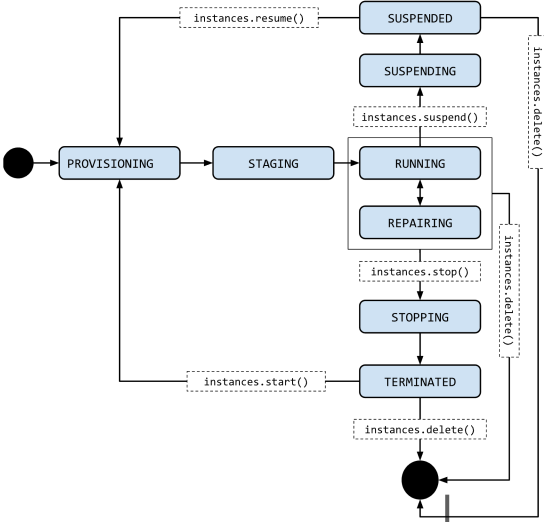
\includegraphics[keepaspectratio]{images/image8.png}}}

\begin{itemize}
\tightlist
\item
  {PROVISIONING}{: Le risorse vengono allocate alla VM che non è ancora
  in esecuzione. Nessun costo in questa fase }
\end{itemize}

{}

\begin{itemize}
\tightlist
\item
  {STAGING}{: Le risorse vengono acquisite dalla VM che si sta
  preparando all\textquotesingle avvio}
\end{itemize}

{}

\begin{itemize}
\tightlist
\item
  {RUNNING}{: La VM è in fase di avvio o esecuzione. Viene eseguito lo
  startup script e avviati tutti i servizi (compreso ssh e rdp)}
\end{itemize}

{}

\begin{itemize}
\tightlist
\item
  {REPAIRING}{: La VM è in fase di riparazione a seguito di un errore
  dell\textquotesingle infrastruttura Google. In questa fase
  l\textquotesingle istanza non è accessibile e non genera costi }
\end{itemize}

{}

\begin{itemize}
\tightlist
\item
  {STOPPING}{: La VM è in fase di arresto, a seguito di errore, azione
  utente o per lo stop di istanze spot}
\end{itemize}

{}

\begin{itemize}
\tightlist
\item
  {TERMINATED}{: La VM è stata arrestata. E\textquotesingle{} possibile
  }{riavviarla}{~o eliminarla }
\end{itemize}

{}

\begin{itemize}
\tightlist
\item
  {SUSPENDING}{: La VM è in fase di sospensione }
\end{itemize}

{}

\begin{itemize}
\tightlist
\item
  {SUSPENDED}{: La VM è in stato di sospensione. E\textquotesingle{}
  possibile ripristinarla o eliminarla.}
\end{itemize}

{}

\subsection{\texorpdfstring{{PaaS - Platform as a
Service}}{PaaS - Platform as a Service}}\label{h.le3mxle0xcus}

{Viene fornita una piattaforma già pronta all'utilizzo per lo sviluppo
software senza la gestione di librerie, S.O., ecc.}

{Scalabile ,sicuro e con un basso Time to market (tempo che va dallo
sviluppo alla commercializzazione di un prodotto).}

{}

\subsection{\texorpdfstring{{SaaS - Software as a Service
}}{SaaS - Software as a Service }}\label{h.hj0y4o2tgbl}

{Servizio più completo e meno personalizzabile, il provider offre un
applicativo fatto e finito utilizzabile con i propri dati e in maniera
isolata; la manutenzione è a carico del provider.}

{}

{Es: Google Suit, Dropbox, Teams\ldots{}}

{}

\section{\texorpdfstring{{Cloud Deployment
Models}}{Cloud Deployment Models}}\label{h.i1clyjht6phv}

{Come il cloud viene implementato cambia da azienda ad azienda oppure la
stessa azienda può avere policy diverse e quindi diverse
implementazioni, per questo esistono 4 modelli di deploy:}

{\pandocbounded{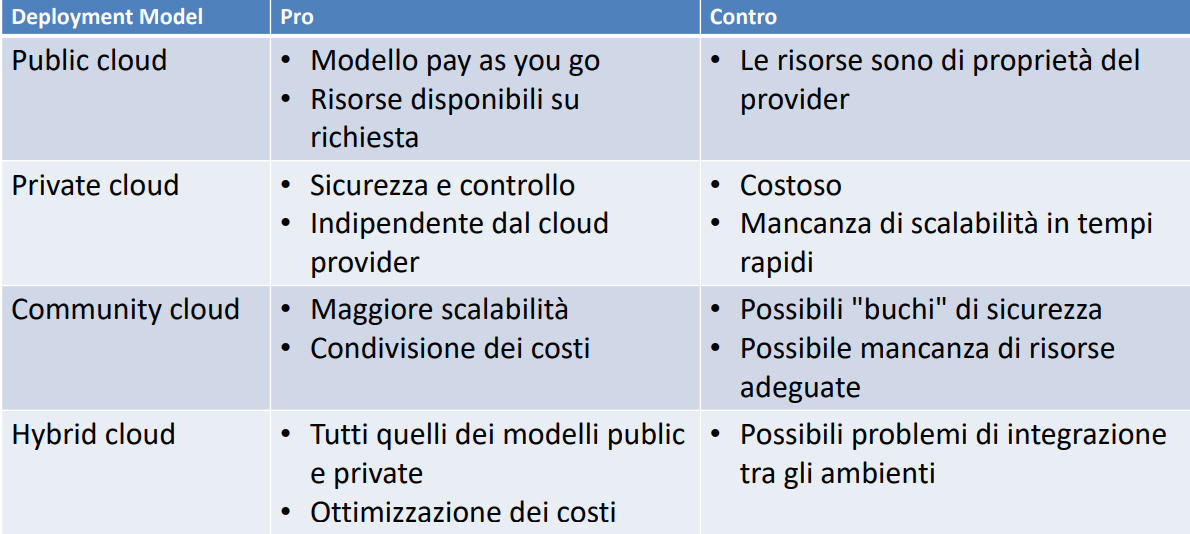
\includegraphics[keepaspectratio]{images/image68.png}}}

{}

\subsection{\texorpdfstring{{Public
Cloud}}{Public Cloud}}\label{h.teu3ij8fh5zi}

{Quello visto fino ad ora, ne fanno parte i Cloud Service Models, dove
chiunque può usare i vari servizi forniti con modalità PAYG.}

{}

\subsection{\texorpdfstring{{Private
Cloud}}{Private Cloud}}\label{h.nflt272axd8u}

{Le risorse fornite sono usate solo da una singola organizzazione per
uso interno, possono essere salvate all'interno della stessa azienda o
ospitate da un provider esterno che ne assicura la protezione e
l'accesso controllato.}

{}

\subsection{\texorpdfstring{{Community
Cloud}}{Community Cloud}}\label{h.rcrd3kdgrf04}

{Più organizzazioni con lo stesso scopo (es: agenzie governative)
condividono un cloud privato andandolo a rendere più flessibile ed
economico come il }{public}{~mantenendo la sua sicurezza.}

{}

\subsection{\texorpdfstring{{Hybrid
Cloud}}{Hybrid Cloud}}\label{h.o9uu245i5d5n}

{Unione del community al }{public}{~con la creazione di due situazioni:}

\begin{itemize}
\tightlist
\item
  {Classic Hybrid Cloud}{: Viene usato il private cloud per i dati e le
  applicazioni proprietarie, ed è usato il public cloud per applicazioni
  non critiche;}
\item
  {Cloud Bursting Hybrid Cloud:}{~Viene principalmente usato il private
  cloud ricorrendo al public cloud solo per gestire i carichi di lavoro
  che eccedono la capacità dell\textquotesingle infrastruttura privata.}
\end{itemize}

{}

{}

\section{\texorpdfstring{{Datacenter}}{Datacenter}}\label{h.jkz5svsorpc2}

{Strutture fisiche dove risiedono tutti componenti che rendono il cloud
funzionante ed efficace come generazione di corrente
(primaria/secondaria), sistemi di raffreddamento e antincendio e
sorveglianza; la ridondanza è obbligatoria per aumentare la tolleranza
ai guasti.}

{}

\subsection{\texorpdfstring{{Struttura
fisica}}{Struttura fisica}}\label{h.sqab6b7kvipj}

{I server e le varie risorse che usano sono aggregate in:}

\begin{itemize}
\tightlist
\item
  {Rack}{: contenente CPU, RAM HDD/SSD ed interfacce di rete, i vari
  rack possono essere inseriti/rimossi in qualsiasi momento in un
  armadio rack.}
\item
  {Blade}{: uguali ai rack per caratteristiche ma più piccoli montati
  sui chassis che alimentano e forniscono connessione ad ogni blade, per
  via delle dimensioni generano più calore.}
\end{itemize}

{}

{Entrambi possono essere aggregati nei }{cluster}{~rendendoli
identificabili come un singolo sistema garantendo }{ridondanza
}{(spostando il lavoro da un server ad un altro senza interruzioni) e
}{modularità}{.}

{}

\subsection{\texorpdfstring{{Connettività}}{Connettività}}\label{h.v6uvagetvlzz}

{Si utilizza la topologia }{Core/Aggregation/Access layers}{~dove ogni
livello ha un compito:}

\begin{itemize}
\tightlist
\item
  {Access: rete con collegamento diretto ai server.}
\item
  {Aggregation: rete per lo smistamento del traffico nelle VLAN.}
\item
  {Core: backbone del datacenter, collega l'aggregation layer con
  l'esterno.}
\end{itemize}

{\pandocbounded{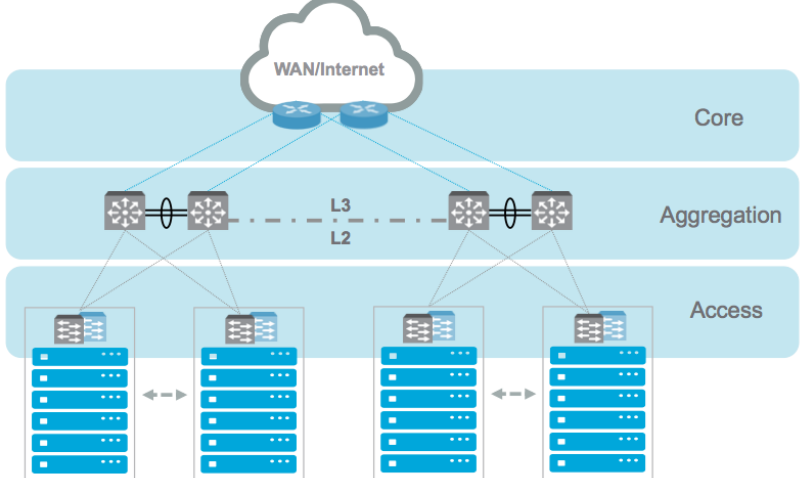
\includegraphics[keepaspectratio]{images/image34.png}}}

{}

{Per la connettività esterna il data center ha uno o più PoP (Point of
Presence), punto importantissimo perché influisce sulla latenza e sulle
prestazioni.}

{}

{}

{}

{Virtualizzazione}

{}

\section{\texorpdfstring{{Tecnologie}}{Tecnologie}}\label{h.5jr9gawl9d8f}

{}

{Nato nel `74 con la pubblicazione del paper: "Formal Requirements for
Virtualizable Third Generation Architectures". }

{L'obiettivo è eseguire sulla stessa macchina fisica più macchine
virtuali (VM) ciascuna:}

\begin{itemize}
\tightlist
\item
  {composta da S.O.}
\item
  {Isolata.}
\item
  {Self contained.}
\item
  {Con risorse condivise.}
\end{itemize}

{}

{\pandocbounded{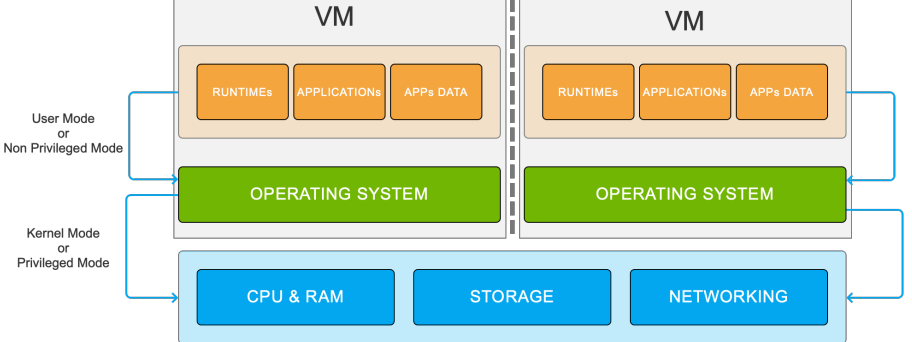
\includegraphics[keepaspectratio]{images/image14.png}}}

{}

{Questo comporta una ottimizzazione dell'utilizzo hardware (meno server
e meno spreco di risorse), riduzione dei costi CapEx e OpEx.}

{}

\section{\texorpdfstring{{Hypervisor}}{Hypervisor}}\label{h.u2kk0jsc3fis}

{Per rendere possibile l'utilizzo contemporaneo di più S.O. è necessario
creare un nuovo strato tra hardware e software detto Hypervisor che
supera il problema di instabilità dato dal Kernel Mode, gestisce e crea
~le VM e le loro risorse.}

{}

{In base a dove posiziono l'Hypervisor cambia il funzionamento e il
tipo:}

\begin{itemize}
\tightlist
\item
  {Type 1 o Bare Metal}{: installato nell'hardware andando a sostituire
  il S.O. rendendolo molto efficiente ed ideale per ambienti server.}
\end{itemize}

{~~~~~~~~Si può classificare in:}

\begin{itemize}
\tightlist
\item
  {Full virtualization o Emulation}{: la VM usa una CPU }{emulata}{~e il
  suo SO pensando si quella vera effettua chiamate in kernel mode che
  vengono intercettate e replicate sull'hardware fisico; l'utilizzo di
  SO standard porta svantaggi ma è comunque possibile.}
\end{itemize}

{}

\begin{itemize}
\tightlist
\item
  {Paravirtualization}{: le VM usano SO modificati che effettuano
  chiamate direttamente all'hypervisor (hypercall) che vengono ripetute
  sull\textquotesingle hardware fisico; migliori performance.}
\end{itemize}

{}

\begin{itemize}
\tightlist
\item
  {Hardware virtualization}{: grazie all'utilizzo di feature i nuovi
  processori possono nativamente dividere e isolare le risorse per ogni
  VM senza quindi l'overhead dell'emulazione.}
\end{itemize}

{}

\begin{itemize}
\tightlist
\item
  {Type 2}{: è un applicativo classico installato su un SO (host os),
  meno efficiente (più mediatori) e adatto ad ambienti desktop.}
\end{itemize}

{}

\section{\texorpdfstring{{Kernel level
virtualization}}{Kernel level virtualization}}\label{h.ms7bwoopd3ky}

{Non è necessario usare un hypervisor grazie al kernel Linux speciale
che gestisce ogni VM come un singolo processo agevolando il ciclo di
vita; ora è possibile la nested virtualization.}

{Usata dal GCP.}

{\pandocbounded{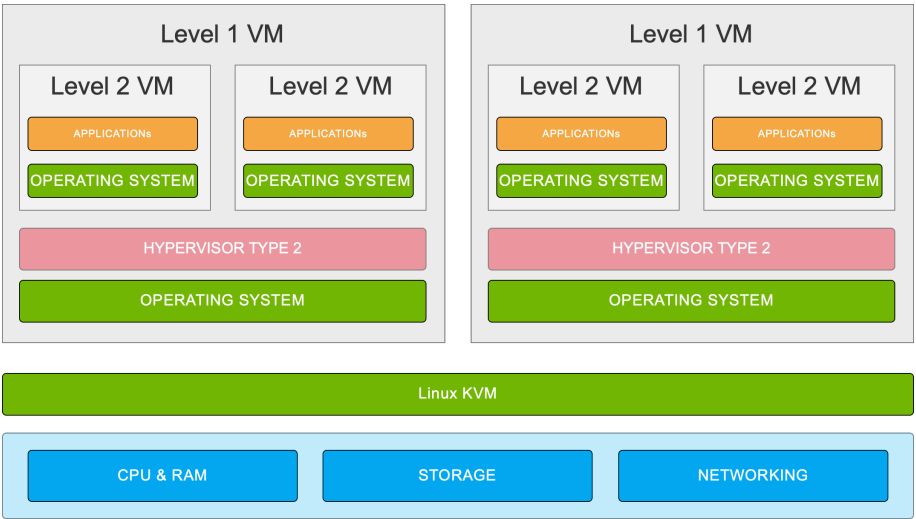
\includegraphics[keepaspectratio]{images/image24.png}}}

\section{\texorpdfstring{{BORG}}{BORG}}\label{h.u6zfxcyoatff}

{Progetto di Google per l'allocazione centralizzata delle risorse dei
data center in maniera scalabile ed efficiente.}

{}

{Tramite un pannello di controllo si gestiscono un intero cluster
assegnando ad ogni worker un task, rispondendo ai cambiamenti nello
stato del cluster e monitorando lo stato di task e worker per riavviare
le operazioni se qualcosa va storto. }

{La scalabilità sta nel fatto che il pannello NON esegue i task
direttamente.}

{}

\section{\texorpdfstring{{OMEGA}}{OMEGA}}\label{h.jtyab6yqqgjz}

{Progetto più recente nato per essere più flessibile e adatto alle nuove
applicazioni come Batch jobs (machine learning), Servizi web con alto
traffico o bassa latenza.}

{}

{~Approccio maggiormente decentralizzato nella gestione dell'allocazione
di risorse dove ogni macchina è responsabile di gestire i propri task e
comunicare con le altre per coordinare l'allocazione di risorse.}

{}

\section{\texorpdfstring{{VPC}}{VPC}}\label{h.y747irz6xg76}

{Virtual Private Cloud (VPC) è il servizio di networking virtuale che
fornisce la connettività alle risorse cloud, tra cui le istanze compute
engine.}

{Essendo create in software non hanno i limiti delle reti fisiche.}

{}

{Esistono solo all'interno dei progetti e nessun progetto non ne può
avere, possono essere condivise.}

{Alla VPC sono associate:}

\begin{itemize}
\tightlist
\item
  {subnet}{: sottoreti con range di indirizzi IPv4 privati associati;}
\item
  {regole di routing}{: per gestire le comunicazioni fra VM di subnet
  diverse;}
\item
  {regole di firewall}{: per gestire traffico in entrata e uscita.}
\end{itemize}

{Le comunicazioni possibili sono mostrate nel grafico:}

{\pandocbounded{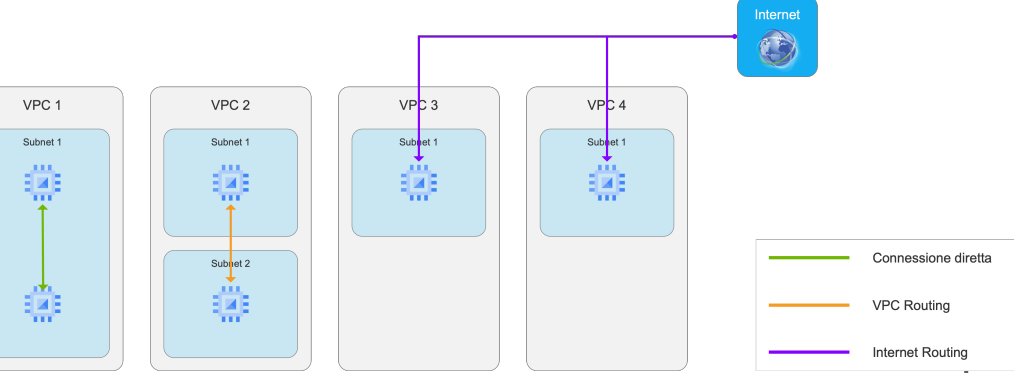
\includegraphics[keepaspectratio]{images/image51.png}}}

{}

{}

{}

{Storage di dati}

\section{\texorpdfstring{{Storage
Pools}}{Storage Pools}}\label{h.n13ihlkevlak}

{i provider offrono diversi tipi di storage che a livello fisico non
sono altro che numerosi HDD o SDD gestiti per comparire come un'unica
entità logica, la gestione può essere fatta in diversi modi:}

{\pandocbounded{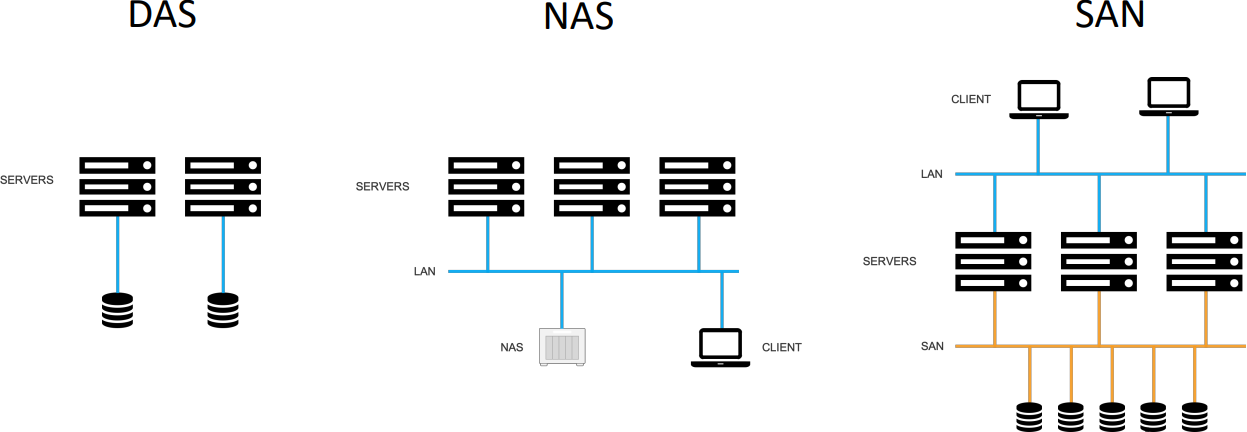
\includegraphics[keepaspectratio]{images/image54.png}}}

{}

\subsection{\texorpdfstring{{DAS - Direct Attached
Storage}}{DAS - Direct Attached Storage}}\label{h.8brrclhcd0jh}

{Dischi fisicamente collegati ad un server tramite connessioni ad alta
velocità e utilizzabili solo al server a cui sono collegati.}

{Questo porta alte prestazioni e bassi costi a scapito della
flessibilità e con un Single Point Of Failure.}

{}

\subsection{\texorpdfstring{{NAS - Network Attached
Storage}}{NAS - Network Attached Storage}}\label{h.mp6lm97garq}

{Dischi collegati tramite rete e accessibili tramite IP, vengono
ospitati in dispositivi con capacità di calcolo e un proprio sistema
operativo per gestire:}

\begin{itemize}
\tightlist
\item
  {policy di accesso}
\item
  {ridondanza RAID}
\item
  {condivisione dati tramite rete}
\end{itemize}

{}

\subsection{\texorpdfstring{{SAN - Storage Area
Network}}{SAN - Storage Area Network}}\label{h.mkgu8ckfe4k7}

{Dischi collegati al server tramite una rete dedicata che utilizza la
fibra, per questo appaiono come dischi locali.}

{Rispetto al DAS sono flessibili e anche resilienti grazie al backup o
snapshot.}

{}

\section{\texorpdfstring{{Data
replication}}{Data replication}}\label{h.dkogd4o06dn3}

{Si tratta di replicare gli stessi dati su più nodi portando ad un
aumento di prestazioni (eliminazione di colli di bottiglia),
disponibilità e sicurezza avendo copie di backup ma anche diminuzione di
latenza portando i dati vicino agli utenti che ne hanno bisogno.}

{}

{Le strategie per replicare sono:}

{}

\subsection{\texorpdfstring{{Full
replication}}{Full replication}}\label{h.gun856a6oe8d}

{Ogni nodo ha una copia di tutto il dataset (ogni nodo è uguale), ottimo
per aumentare le performance di lettura e la sicurezza ma pessimo per la
scrittura visto che le modifiche dovranno essere propagate a tutti i
nodi (portando ad un overhead sulla rete e maggiori tempi di
esecuzione).}

{}

\subsection{\texorpdfstring{{Partial
replication}}{Partial replication}}\label{h.b0o98mp8l9oe}

{Solo alcuni nodi hanno le repliche portando ad una propagazione delle
modifiche più snella.}

{Diminuiscono le performance visto che dovrò cercare il nodo specifico e
la sicurezza (meno backup).}

{}

\subsection{\texorpdfstring{{Consistenza}}{Consistenza}}\label{h.8ejqij3ki14k}

{In entrambe le strategie si genera il problema
dell\textquotesingle inconsistenza dei dati perché bisogna garantire che
tutte le repliche siano uguali.}

{Per risolvere abbiamo due approcci:}

\subsubsection{\texorpdfstring{{Strong
consistency}}{Strong consistency}}\label{h.ldxh5fqezegb}

{In ogni istante tutti i nodi sono uguali, per questo si bloccano tutte
le operazioni fino a propagazione conclusa, con degrado rapido delle
performance.}

\subsubsection{\texorpdfstring{{Weak
consistency}}{Weak consistency}}\label{h.1k85zznzkf9t}

{In questo caso le operazioni sui nodi sono possibili nonostante la
propagazione delle modifiche, questo può portare ad inconsistenza e
corruzione ma le performance non ne risentono.}

{}

\subsection{\texorpdfstring{{Read
replicas}}{Read replicas}}\label{h.5ledo7sne0rx}

{Si utilizza una copia primaria su cui effettuare sia le operazioni di
lettura che di scrittura e una o più copie secondarie su cui effettuare
solo le operazioni di lettura.}

{}

\section{\texorpdfstring{{Tipologie di
storage}}{Tipologie di storage}}\label{h.mj3sf1rv45bx}

{Un public cloud provider offre alcuni se non tutti questi storage:}

{}

\subsection{\texorpdfstring{{Block
Storage}}{Block Storage}}\label{h.6q25hzblffb8}

{Viene memorizzato tutti in strutture di dimensioni fissa (block) in
questo tipo di storage vengono installati software o SO che richiedono
accesso diretto a questi block.}

{Utilizzato da VM per il boot disk e secondary disk.}

{}

\subsection{\texorpdfstring{{File
Storage}}{File Storage}}\label{h.vqmv8duwo3z9}

{Forniscono file system accessibili via rete e servono per realizzare
soluzioni NAS (vedi su), sono indipendenti rispetto al file system delle
VM garantendo condivisione di file tra più applicazioni.}

{}

\subsection{\texorpdfstring{{Object
Storage}}{Object Storage}}\label{h.n96nm2ffnlb7}

{Dati memorizzati in termini di Oggetti o Blob, che di solito sono file,
ma in maniera non analoga ad un file system (cartelle).}

{}

{Ogni oggetti ad un indirizzo con cui si può accedere anche senza VM;
l\textquotesingle accesso è pubblico o gestito da policy.}

{Gli oggetti sono solo sovrascrivibili ed è possibile avere una
storicizzazione delle versioni.}

{}

{\pandocbounded{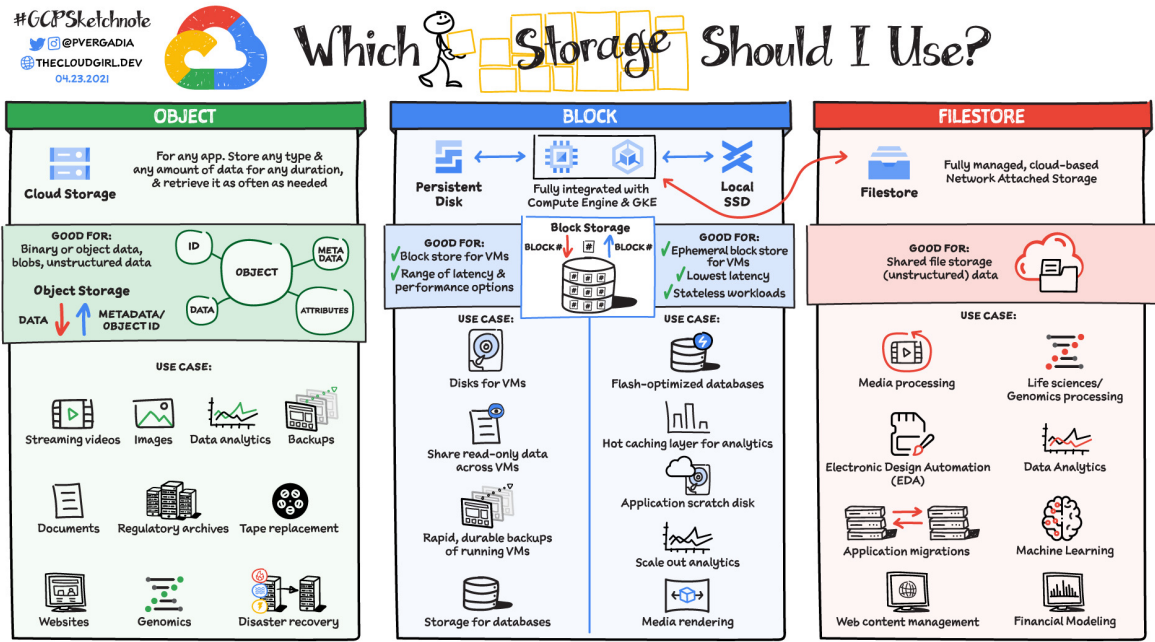
\includegraphics[keepaspectratio]{images/image44.png}}}

{}

\subsection{\texorpdfstring{{Cache}}{Cache}}\label{h.969uz64ih2s4}

{I dati vengono mantenuti qui per un accesso rapido e con latenze
\textless{} del millisecondo; ma essendo volatili ad un riavvio del
server i dati, a meno che non siano salvati nel system of truth, vengono
persi.}

{}

{Capita che vadano fuori sync rispetto al system of truth, se le
modifiche non vengono replicate correttamente.}

{}

\subsection{\texorpdfstring{{Database}}{Database}}\label{h.4qqytg3pm9uo}

{Un Database Management System (DBMS) è una applicazione che si occupa
della memorizzazione e gestione dei dati, con le seguenti
caratteristiche: }

\begin{itemize}
\tightlist
\item
  {Gestisce grandi quantità di dati con particolare attenzione
  all'efficienza. }
\item
  {Gestisce la persistenza dei dati garantendo la fault tolerance. }
\item
  {Gestisce la condivisione dei dati garantendo il controllo degli
  accessi e della concorrenza}
\item
  {Definisce uno o più linguaggi di programmazione per interagire con i
  dati }
\item
  {Divide lo schema fisico dallo schema logico }
\item
  {Prevede uno o più sistemi per effettuare il backup e il ripristino
  dei dati }
\item
  {Può prevedere la possibilità di replicare i dati su più server, per
  aumentare la disponibilità e le prestazioni}
\end{itemize}

{}

{I DBMS sono classificati in due famiglie:}

{\pandocbounded{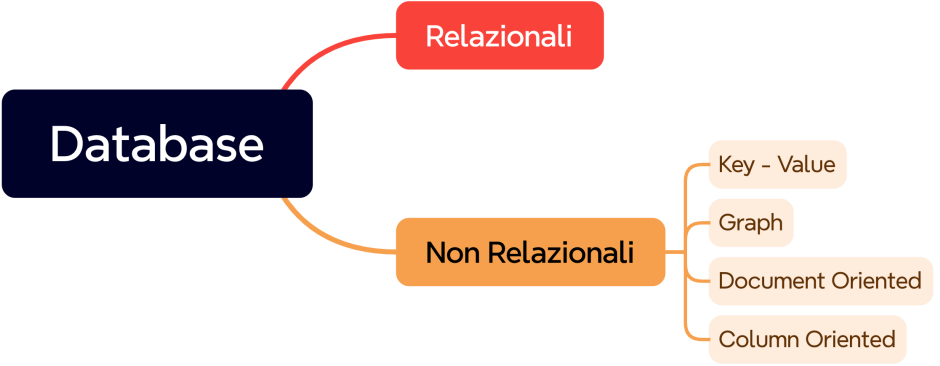
\includegraphics[keepaspectratio]{images/image25.png}}}

\subsubsection{\texorpdfstring{{Relazionali}}{Relazionali}}\label{h.y25e56io9v9d}

{I dati sono modellati tramite il concetto di Relazione rappresentato in
forma tabellare, dove ad ogni occorrenza di dominio si associa un nome
univoco, detto attributo. Questo permette di aumentare la leggibilità,
di migliorare l\textquotesingle espressività e di rendere irrilevante
l'ordine con cui si considerano i domini. Ad ogni relazione è inoltre
associato un nome univoco.}

{\pandocbounded{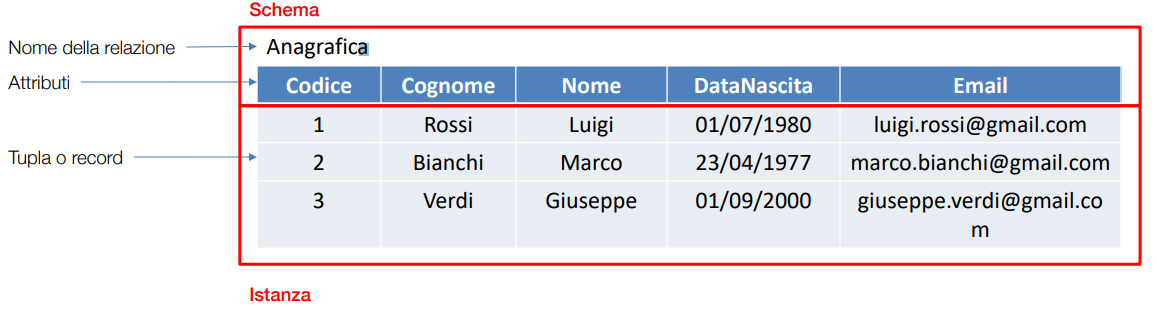
\includegraphics[keepaspectratio]{images/image69.png}}}

{Per essere considerati validi i dati devono seguire dei vincoli di
integrità, cioè, proprietà che deve essere soddisfatte dalle istanze.}

{}

{Tutta la parte dei vincoli
}{\href{https://www.google.com/url?q=https://virtuale.unibo.it/pluginfile.php/2015119/mod_resource/content/1/Lezione\%25203\%2520-\%2520Storage\%2520dei\%2520dati.pdf&sa=D&source=editors&ust=1734628634268296&usg=AOvVaw2c0HDBkCyOu4HrDZixCKja}{QUI}}{~(slide
38 - 43)}

{}

{Per lavorare sulle tabelle si usa un linguaggio dichiarativo detto SQL
che tramite query è possibile fare le seguenti operazioni:}

\begin{itemize}
\tightlist
\item
  {DDL }{- Data Definition Language: Per creare/modificare/cancellare
  database e tabelle }
\end{itemize}

{}

\begin{itemize}
\tightlist
\item
  {DML }{- Data Manipulation Language: Per interrogare e modificare i
  dati presenti nelle tabelle }
\end{itemize}

{}

\begin{itemize}
\tightlist
\item
  {DCL }{- Data Control Language: Per gestire i diritti di accesso degli
  utenti alle tabelle}
\end{itemize}

{}

{Il vantaggio di questo modello è il concetto di }{transazione}{, cioè
l'insieme di operazioni correlate secondo la proprietà }{ACID}{:}

\begin{itemize}
\tightlist
\item
  {Atomicity}{: Una transazione è atomica, ovvero è trattata come
  un\textquotesingle unità indivisibile. In caso di errore
  l\textquotesingle intera transazione viene annullata (rollback)}
\end{itemize}

{}

\begin{itemize}
\tightlist
\item
  {Consistency}{: La transazione lascerà il database sempre in uno stato
  consistente}
\end{itemize}

{}

\begin{itemize}
\tightlist
\item
  {Isolation}{: Le transazioni in esecuzione concorrente non
  interferiscono tra di loro}
\end{itemize}

{}

\begin{itemize}
\tightlist
\item
  {Durability}{: L\textquotesingle effetto di una transazione terminata
  con successo è permanente. }
\end{itemize}

{}

\subsubsection{\texorpdfstring{{Non
relazionali}}{Non relazionali}}\label{h.xnccng3k9z76}

{Non usano le relazioni per modellare i dati e ne esistono di più tipi:
}

\begin{itemize}
\tightlist
\item
  {Key-Value: dati archiviati in vettori ciascuno acceduto da una
  specifica chiave}
\end{itemize}

{}

\begin{itemize}
\tightlist
\item
  {Graph: dati rappresentati in termini di entità e relazioni tra loro,
  molto usati per social network o strumenti di analisi}
\end{itemize}

{}

\begin{itemize}
\tightlist
\item
  {Document Oriented: modello in cui ogni dato è trattato come un
  documento JSON che può essere annidato ad altri in maniera gerarchica}
\end{itemize}

{}

\begin{itemize}
\tightlist
\item
  {Column Oriented: dati archiviati in tabelle con colonne che variano
  dinamicamente in base alle tipologie di dati}
\end{itemize}

{}

{Non imponendo uno schema rigido e vincolato, risultano più performanti
ma non garantiscono allo stesso modo l\textquotesingle integrità dei
dati. Hanno alcune caratteristiche comuni:}

\begin{itemize}
\tightlist
\item
  {Basically Available}{: garantisce che il database risponderà alle
  richieste, ma non per forza con la versione dei dati più recente }
\item
  {Soft}{-}{state}{: lo stato del database può cambiare nel tempo anche
  senza input (esempio per sincronizzare dati) }
\item
  {Eventually consistent}{: il database non sarà subito consistente.
  Potrebbero esserci ritardi tra le operazioni di scrittura e la loro
  sincronizzazione su tutte le repliche}
\end{itemize}

{}

\section{\texorpdfstring{{Storage
GCP}}{Storage GCP}}\label{h.vuxbuojz5nrk}

{Le categorie viste in precedenza, anche se con nomi diversi, vengono
offerti come servizi da GCP, eccoli:}

{\pandocbounded{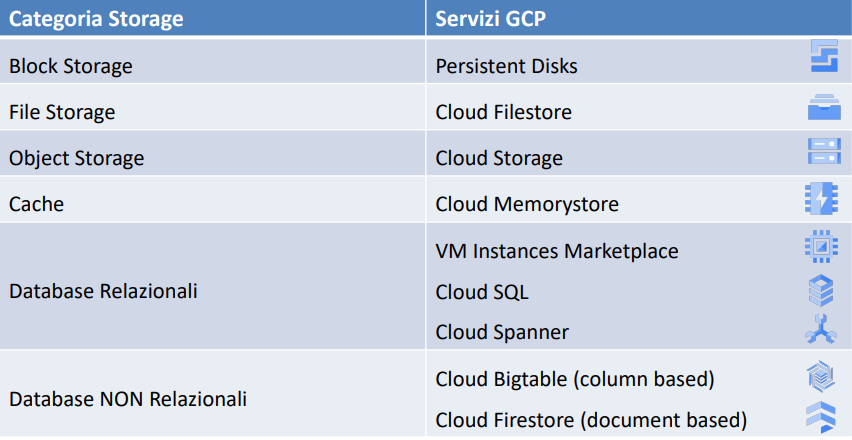
\includegraphics[keepaspectratio]{images/image65.png}}}

{Vediamone alcuni:}

{}

\subsection{\texorpdfstring{{Cloud
Filestore}}{Cloud Filestore}}\label{h.7vbm23dqsio}

{Servizio di NAS utilizzabile con VM o cluster Kubernetes, utilizza
NFSv3 per usare i filesystem di rete con performance alte adatte a
carichi di lavoro intensivi. Scalabile fino a 100TB.}

{}

\subsection{\texorpdfstring{{Cloud
Storage}}{Cloud Storage}}\label{h.hohi95du92ba}

{\pandocbounded{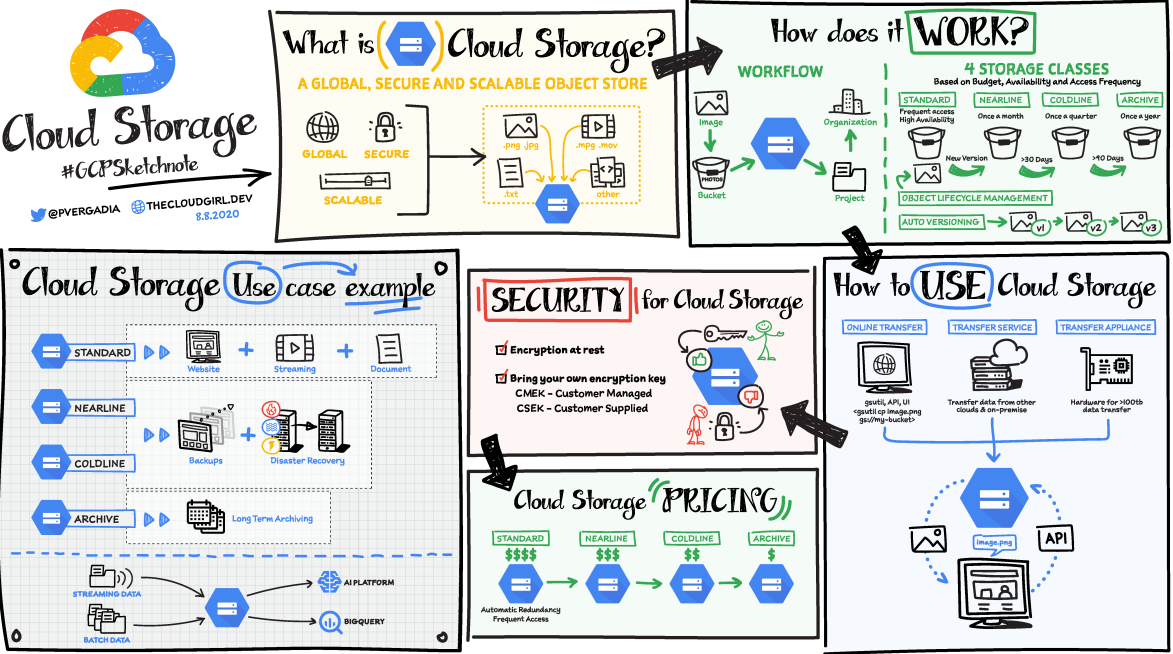
\includegraphics[keepaspectratio]{images/image5.png}}}

{Servizio Object Storage con oggetti di qualsiasi tipo, immutabili e
organizzati in bucket univoci a livello globale; è possibile avere uno
storico delle versioni precedenti (identificati da un numero di
generazione).}

{}

{Oggetti accessibili tramite policy e url univoco.}

{}

{Cloud storage è adatto a memorizzare oggetti gestiti come una "unica
unità", ovvero oggetti che vengono sempre letti e scritti nella loro
interezza. Non è adatto ad oggetti che richiedono un accesso parziale.}

{}

{Può essere regionale o multiregionale, spazio scalabile all'infinito.}

{I dati possono essere archiviati in 4 classi di archiviazione, che
differiscono per tempi di accesso e per costi: }

\begin{itemize}
\tightlist
\item
  {Standard: È la classe da utilizzare per accessi frequenti }
\item
  {Nearline: È la classe per accessi che avvengono una volta al mese }
\item
  {Coldline: È la classe per accessi che avvengono una volta ogni 90
  giorni }
\item
  {Archive: È la classe per accesso che avvengono una volta
  all\textquotesingle anno }
\end{itemize}

{}

{Le classi Nearline, Coldline e Archivie, oltre al costo per lo spazio
utilizzato, prevedono un costo per ogni singolo accesso. La classe può
essere cambiata per ogni oggetto anche in maniera automatica tramite
policy dette }{lifecycle management}{.}

{}

\subsection{\texorpdfstring{{Cloud
Memorystore}}{Cloud Memorystore}}\label{h.qdz31hamgsmw}

{È il servizio di cache in-memory, per aumentare le performance di
accesso ai dati più frequentemente usati }

{Supporta due dei principali sistemi open source di caching: }

\begin{itemize}
\tightlist
\item
  {Redis }
\item
  {Memcached }
\end{itemize}

{È sufficiente specificare la dimensione della cache, lasciando alla
piattaforma la gestione di tutti gli aspetti amministrativi}

{\pandocbounded{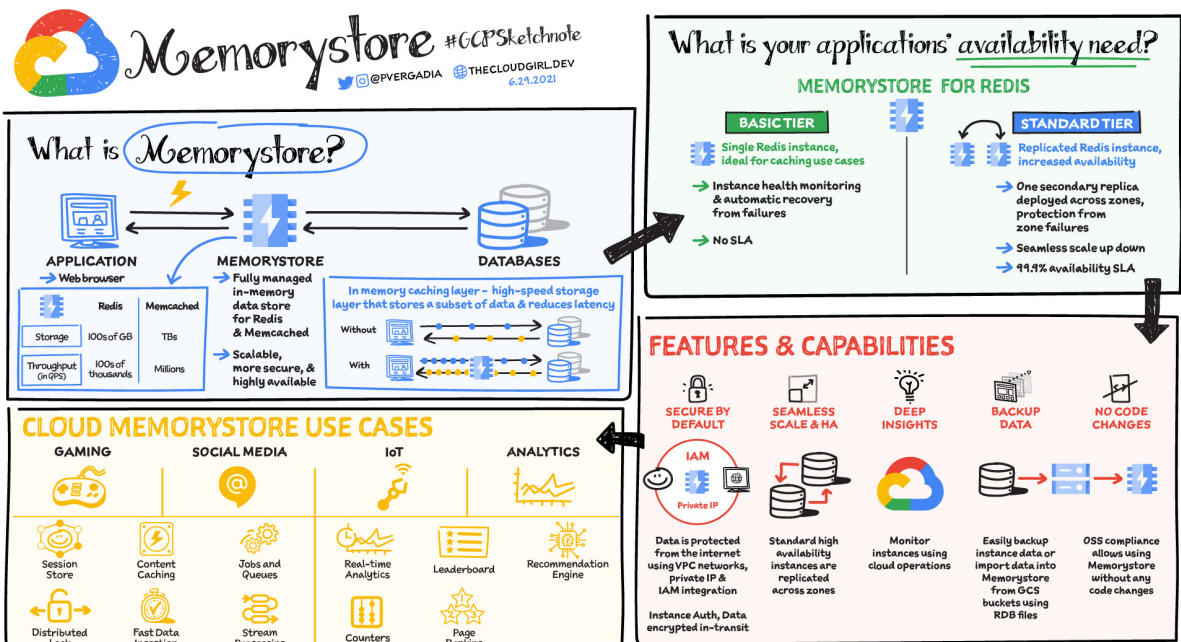
\includegraphics[keepaspectratio]{images/image6.png}}}

{}

\subsection{\texorpdfstring{{Cloud
SQL}}{Cloud SQL}}\label{h.2931p5qzdx31}

{È il servizio che mette a disposizione i principali DBMS relazionali in
modo completamente gestito da Google.}

{}

{Le attività di amministrazione, quali backup, aggiornamenti e gestione
del failover sono completamente gestite da Google.
L\textquotesingle unica attività amministrativa necessaria riguarda la
definizione degli utenti e dei relativi diritti di accesso.}

{}

{Progettato per gestire le repliche ed essere a bassa latenza, dati
crittografati at-rest e in-transit.}

{La replica è gestita tramite istanza primaria e fino a 10 istanze
secondarie in sola lettura e ospitate in: }

\begin{itemize}
\tightlist
\item
  {Stessa }{region}{~ma zona differente (Read Replica) }
\item
  {Region differente (Cross Region Read Replica) }
\item
  {On Premises (External Replica) }
\end{itemize}

{}

{Le repliche possono essere "promosse" a istanza primaria, con eccezione
delle External Replica.}

{La loro utilità sta nei seguenti scenari:}

\begin{itemize}
\tightlist
\item
  {Aumentare le performance, dividendo il carico di lettura tra tutte le
  repliche }
\item
  {Migrare database da una }{region}{~ad un\textquotesingle altra,
  creando una nuova replica nella nuova }{region e}{~promuovendo a
  istanza principale }
\item
  {Gestire la High Availability, promuovendo una replica ad istanza
  primaria in caso di fallimento dell\textquotesingle attuale}
\end{itemize}

{}

{\pandocbounded{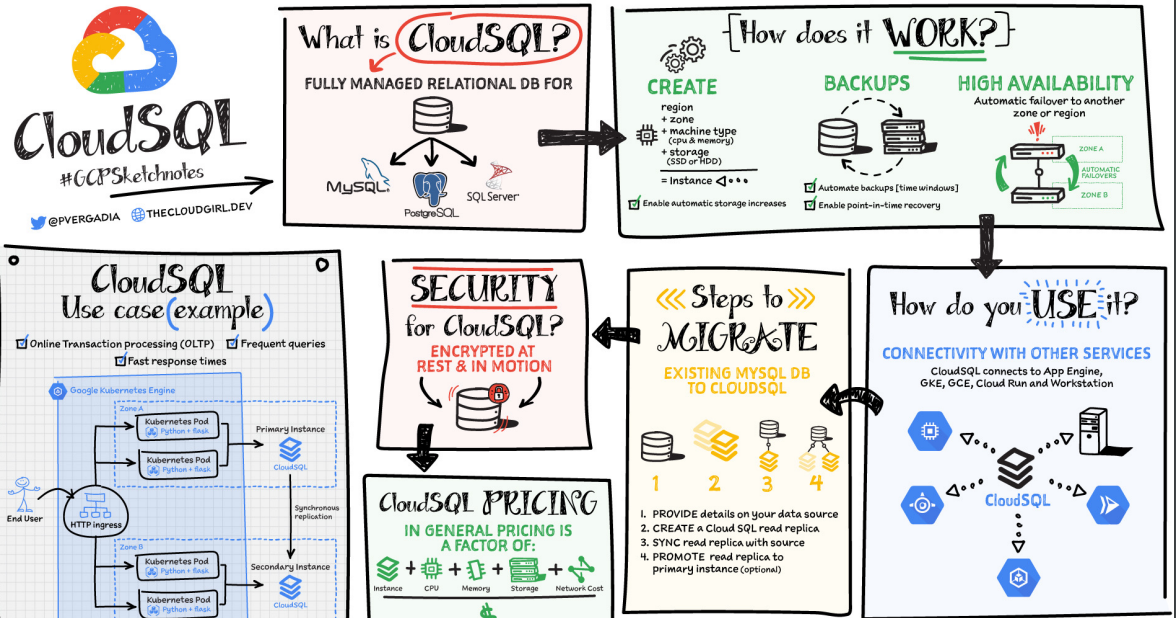
\includegraphics[keepaspectratio]{images/image63.png}}}

{}

\subsection{\texorpdfstring{{Cloud
Spanner}}{Cloud Spanner}}\label{h.kqow4elpup59}

{È il database relazionale "cloud-native" e distribuito globalmente,
combina i vantaggi dei database relazionali e di quelli noSQL: }

\begin{itemize}
\tightlist
\item
  {Forte consistenza dei dati }
\item
  {Transazioni ACID }
\item
  {Scalabilità orizzontale (repliche)relazionale "cloud-native" e
  distribuito globalmente.}
\end{itemize}

{}

{Come Cloud SQL c'è la crittografia at-rest e in-transit, supporta
comunque SQL standard.}

{\pandocbounded{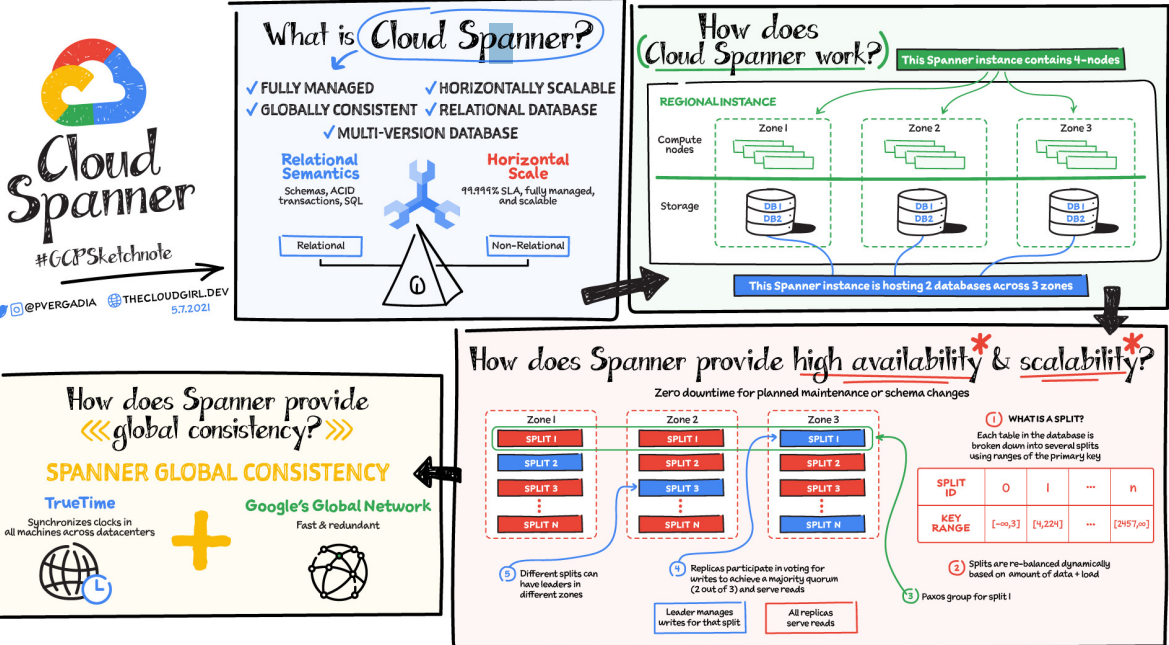
\includegraphics[keepaspectratio]{images/image27.png}}}

{}

\subsection{\texorpdfstring{{Cloud
Bigtable}}{Cloud Bigtable}}\label{h.md39y53i5yvl}

{Servizio completamente gestito di database NoSql column based perfetto
per la gestione di Terabyte e Petabyte di dati, garantendo bassa latenza
e alto throughput; non prevede le transazioni per cui deve essere usato
in contesti in cui non c\textquotesingle è tale necessità }

{È un servizio regionale con la possibilità di replica automatica dei
dati.}

{}

{Scala orizzontalmente in maniera automatica, pensato per applicazioni
real time e analisi di dati.}

{}

\subsection{\texorpdfstring{{Cloud
Firestore}}{Cloud Firestore}}\label{h.bena0iz01deo}

{È un servizio di database NoSql basato su documenti. progettato per
essere real time, avere alte performance e per scalare automaticamente.
}

{Gestisce le transazioni e prevede un linguaggio di interrogazione SQL
Like precedentemente noto come Cloud Datastore, e può essere configurato
in modalità Datastore.}

{\pandocbounded{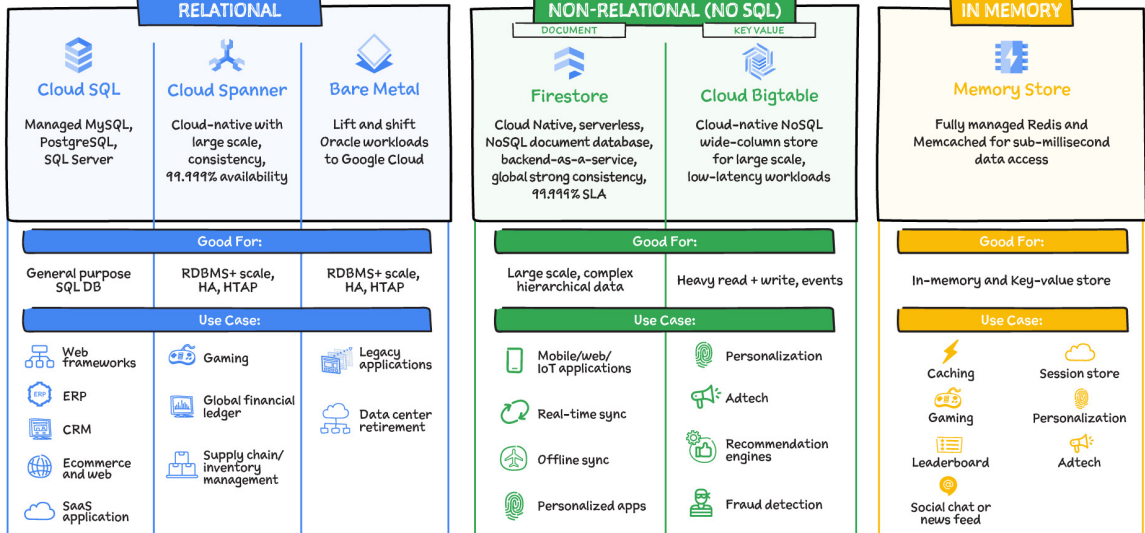
\includegraphics[keepaspectratio]{images/image17.png}}}

{}

{Scalable Computing}

\section{\texorpdfstring{{Scalabilità}}{Scalabilità}}\label{h.fm3ludyfgpci}

{Si intende l'aggiunta di risorse in un ambiente di lavoro per adeguarlo
al carico di lavoro (rapid elasticity), la scalabilità può essere
verticale/orizzontale.}

{}

\subsection{\texorpdfstring{{Verticale}}{Verticale}}\label{h.jmzpm1zd0cl9}

{Scalabilità molto versatile e applicabile a qualsiasi applicazione,
dove si potenzia semplicemente il numero di risorse già esistenti
(aumento di }{vCPU}{~e RAM).}

{La versatilità si paga con il dover riavviare una risorsa prima di
poterle cambiare configurazione o lo spreco di risorse dovuto ad una
diminuzione di risorse non tempestiva.}

{}

\subsection{\texorpdfstring{{Orizzontale}}{Orizzontale}}\label{h.74ptrt438l78}

{In questo caso si duplicano le risorse (creazione di una seconda VM
uguale alla prima) andando poi a dividere il lavoro. }

{}

{Questo tipo di scalabilità non è possibile con le applicazioni che
mantengono uno stato applicativo, applicazione }{stateful}{, visto che
la duplicazione creerebbe copie degli stessi dati con successivo
disallineamento.}

{Per questo esistono le applicazioni }{stateless}{, perfette per la
scalabilità orizzontale, dove non c'è nessun tipo di dato gestito (come
una webapp che eroga solo HTML / CSS senza un backend).}

{}

{L'applicazione stateful può essere scalata orizzontalmente andando a
centralizzare lo stato applicativo, condividendolo con tutte le
istanze.}

{}

\subsection{\texorpdfstring{{Horizontal
Autoscaling}}{Horizontal Autoscaling}}\label{h.2xd9muwm437}

{Quando il provider scala in automatico orizzontalmente una risorsa
tramite policy }{definite dall'utente,}{~normalmente su delle soglie.}

{La scalabilità avviene su gruppi di risorse, es: gruppo di VM dove se
ne aggiunge una nuova. }

{}

{In GCP si chiama Managed Instance Group}{, dove si crea un set di VM
identiche detto }{instance group}{~che può essere:}

\begin{itemize}
\tightlist
\item
  {Managed (MIG)}{: configurati per scalare automaticamente
  orizzontalmente e per bilanciare il traffico tra le istanze; si
  possono creare zonal MIG (tutte le istanze nella stessa zona) o
  regional MIG (istanze sparse su una regione e più resilienti).}
\end{itemize}

{}

\begin{itemize}
\tightlist
\item
  {Unmanaged}{: le VM appartenenti al gruppo possono essere differenti
  tra di loro e per questo l'istanza va creata manualmente e anche le
  varie scalature.}
\end{itemize}

{}

{Quando si configura l'autoscaling delle }{MIG }{bisogna tenere conto i
tempi di boot/shutdown delle VM, infatti se il tempo tra due controlli
di autoscaling è troppo piccolo ci si può trovare nella situazione in
cui una VM appena aggiunta non è ancora completamente operativa
(aggiunta non voluta di più istanze).}

{}

{Le }{MIG}{~effettuano degli }{health checks}{, dove si mantengono in
running le istanze e si riavviano VM bloccate, con anche aggiornamenti a
rotazione per evitare che tutte le VM si blocchino nello stesso momento
per aggiornare.}

{}

\section{\texorpdfstring{{Reverse
Proxy}}{Reverse Proxy}}\label{h.57nlkjq4lqj4}

{Andando a scalare orizzontalmente si crea il problema dell'accesso
diverso ad ogni istanza, infatti sarebbe opportuno avere un indirizzo IP
per ogni VM e informare i client di tutti i nuovi IP ad ogni scaling.}

{Per questo è nato il reverse proxy, un intermediario che accetta tutte
le richieste in entrata dai client e restituisce le varie risorse
andandole a prendere dalle varie istanze senza che il cliente sappia da
chi arriva la risposta; il proxy dovrà sempre sapere quante sono le VM e
quindi informato ad ogni scalo orizzontale.}

{\pandocbounded{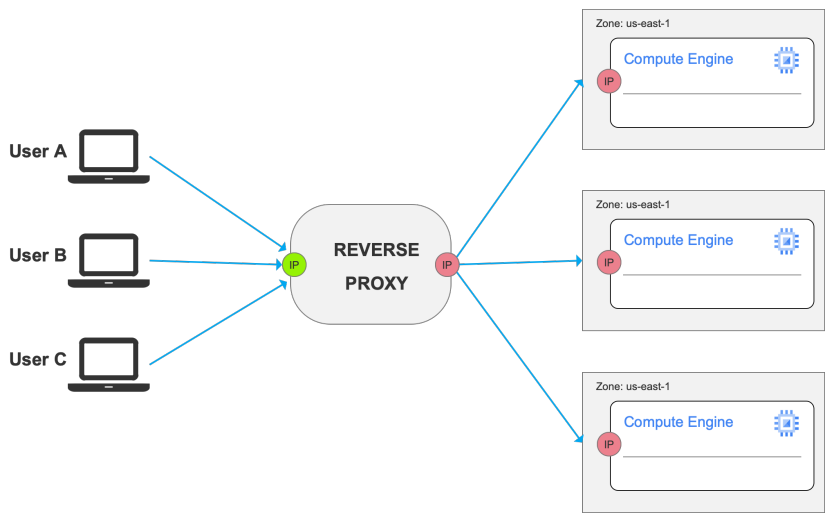
\includegraphics[keepaspectratio]{images/image58.png}}}

{Es: Nginx e Apache}

{}

{Il proxy sarà l'unico ad avere IP pubblico andando a migliorare la
sicurezza, gestendo i vari accessi ed eventualmente effettuare
elaborazioni sul traffico.}

{}

{La connessione tra client e VM essendo intermediata dal proxy viene
divisa in due e sarà proprio lui ad effettuare la terminazione della
connessione.}

{\pandocbounded{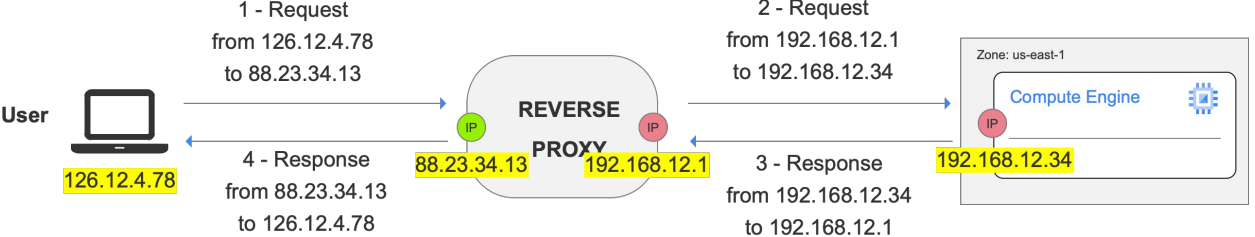
\includegraphics[keepaspectratio]{images/image57.png}}}

{}

{Il reverse proxy presenta anche dei limiti come:}

\begin{itemize}
\tightlist
\item
  {Single point of Failure}{: In caso di malfunzionamento
  l\textquotesingle intero sistema diventa irraggiungibile }
\item
  {Scalabilità limitata}{: può scalare solo verticalmente}
\item
  {Complessità}
\item
  {Latenza aggiuntiva}
\end{itemize}

{}

\subsection{\texorpdfstring{{Load
Balancing}}{Load Balancing}}\label{h.slhea69ack73}

{È il processo effettuato da un proxy per distribuire il traffico di
rete verso molteplici server, garantendo che nessuno sia sovraccarico,
ottimizzando le risorse, garantendo il minor tempo di risposta e il
massimo throughput.}

{Il load balancing è applicabile tramite }{software}{~(algoritmo
aggiunto al proxy tramite app) oppure }{hardware}{~(componenti fisici
installati in un data center).}

{}

{Per farlo sono stati creati alcuni algoritmi che differiscono in base
alla scelta a chi indirizzare le richieste.}

\subsubsection{\texorpdfstring{{Round
Robin}}{Round Robin}}\label{h.j8nlwwvpwq60}

{Algoritmo semplice, basilare e senza garanzie che manda le richieste in
maniera sequenziale senza controlli sul carico di lavoro o connessioni
attive.}

\subsubsection{\texorpdfstring{{Least
Connection}}{Least Connection}}\label{h.wt41en6epydx}

{La richiesta viene inoltrata al server con meno richieste all'attivo,
quindi si prova a bilanciare le richieste su tutti i server.}

{Ottimo in ~scenari in cui le connessioni hanno tutte circa lo stesso
numero di richieste, ma meno adatto a scenari più dinamici.}

\subsubsection{\texorpdfstring{{Altri}}{Altri}}\label{h.ylbbgtvc5jxa}

\begin{itemize}
\tightlist
\item
  {Least Response Time}{: Le richieste sono inoltrate al server con
  minor tempo di risposta }
\end{itemize}

{}

\begin{itemize}
\tightlist
\item
  {Weighted Round Robin:}{~Analogo al RR, ma ad ogni server viene
  assegnato un peso, ovvero una \% di richieste che deve ricevere}
\end{itemize}

{}

\begin{itemize}
\tightlist
\item
  {Random}{: Inoltra le richieste in modo completamente randomico }
\end{itemize}

{}

\begin{itemize}
\tightlist
\item
  {IP Hash}{: Inoltra le richieste provenienti dallo stesso client
  sempre allo stesso server, in modo da poter gestire localmente la
  sessione }
\end{itemize}

{}

\begin{itemize}
\tightlist
\item
  {Adaptive}{: Valutano molteplici aspetti del server (carico,
  connessioni, response time\ldots)}
\end{itemize}

\subsubsection{\texorpdfstring{{Cloud Load
Balancer}}{Cloud Load Balancer}}\label{h.83w2dgohryv1}

{Soluzione offerta dai provider dove l\textquotesingle utente non deve
gestire nulla, basta configurarlo in termini di protocolli da usare,
algoritmo, porte, e su quali server bilanciare.}

\subsubsection{\texorpdfstring{{Google Load
Balancing}}{Google Load Balancing}}\label{h.9j9m68b5t7eu}

{Sono servizi distribuiti globalmente ed interamente gestiti in software
da Google. Non si richiedono configurazioni hardware né la creazione di
VM dedicate; con }{autoscaling}{~e l\textquotesingle health check
utilizzando managed instance group come backend.}

{}

{GCP ne prevede 6 tipologie combinate in quattro dimensioni:}

\begin{itemize}
\tightlist
\item
  {Global }{vs Regional}{:}{~i globali usano EDGE Network, erogati dai
  EDGE POP, usati se gli utenti sono sparsi.}
\end{itemize}

{I regionali distribuiscono il traffico verso istanze che si trovano
tutte nella stessa }{region.}

{}

\begin{itemize}
\tightlist
\item
  {External }{vs Internal:}{~i primi smistano il traffico proveniente
  dalla Internet pubblica e diretto alle istanze interne a GCP, i
  secondi }{smistano}{~solamente traffico interno alla rete di Google.}
\end{itemize}

{}

\begin{itemize}
\tightlist
\item
  {Proxy vs Passthrough}{: I load balancer proxy interrompono le
  connessioni in entrata e aprono nuove connessioni dal bilanciatore ai
  backend. I backend risponderanno quindi al LB che inoltrerà le
  risposte al client. I load balancer passthrough non interrompono le
  connessioni e si limitano ad inoltrare i pacchetti a destinazione.}
\end{itemize}

{\pandocbounded{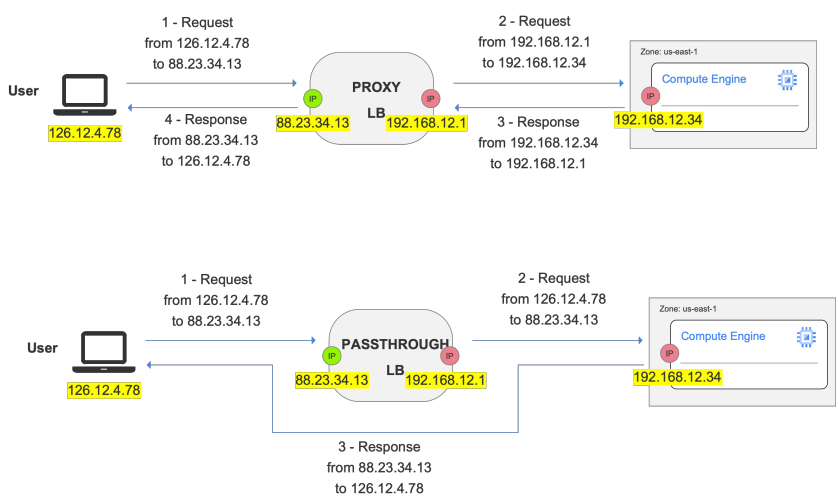
\includegraphics[keepaspectratio]{images/image1.png}}}

{}

{I load balancer di GCP si differenziano per il tipo di traffico che
possono gestire e inoltrare:}

{\pandocbounded{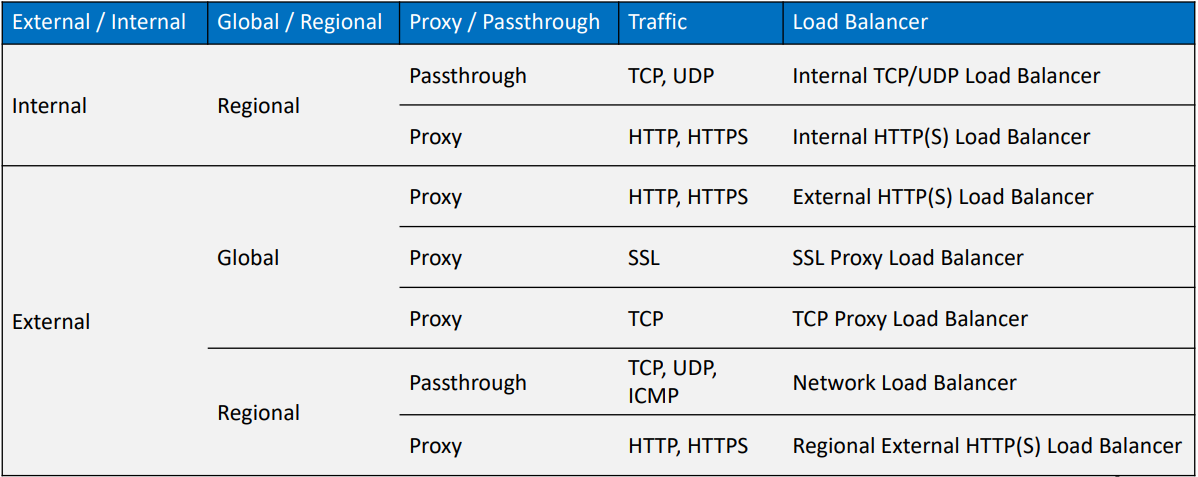
\includegraphics[keepaspectratio]{images/image12.png}}}

{}

\section{\texorpdfstring{{CDN}}{CDN}}\label{h.izyx4tup6x19}

{O Content Delivery Network, sistema di caching e indirizzamento di
client verso il nodo più vicino per evitare sovraccarichi di rete e
attese troppo lunghe. }

{L'idea è nata perché un utente che accede a dei dati probabilmente
}{accederà}{~ad altri dati logicamente simili e può }{riaccedere}{~allo
stesso dati più volte in un breve lasso di tempo.}

{}

{Ogni CDN è composto da:}

\begin{itemize}
\tightlist
\item
  {Origin Server}{: dove si trovano i dati da consegnare.}
\end{itemize}

{}

\begin{itemize}
\tightlist
\item
  {CDN Server}{: dove si mantengono i dati forniti
  dall\textquotesingle origin server e distribuiti in posizioni tali da
  limitare la latenza. Questi dati non vengono copiati in modo
  sistematico ma è fatto quando il client lo richiede, possono avvenire
  due casistiche:}
\end{itemize}

\begin{enumerate}
\tightlist
\item
  {Cache Miss}{: il contenuto non è nel CDN e si richiede.}
\item
  {Cache Hit}{: il contenuto è già nel CDN e si invia.}
\end{enumerate}

{I contenuti in cache possono essere cancellati dopo un tot di tempo
(tramite TTL) e si dice }{Cache TTL}{~o si svuota la cache a necessità
(}{Cache Invalidation}{).}

{}

\begin{itemize}
\tightlist
\item
  {DNS }{Redirection}{: per risolvere il nome di dominio con
  l\textquotesingle indirizzo IP del CDN Server più vicino al client.}
\end{itemize}

{\pandocbounded{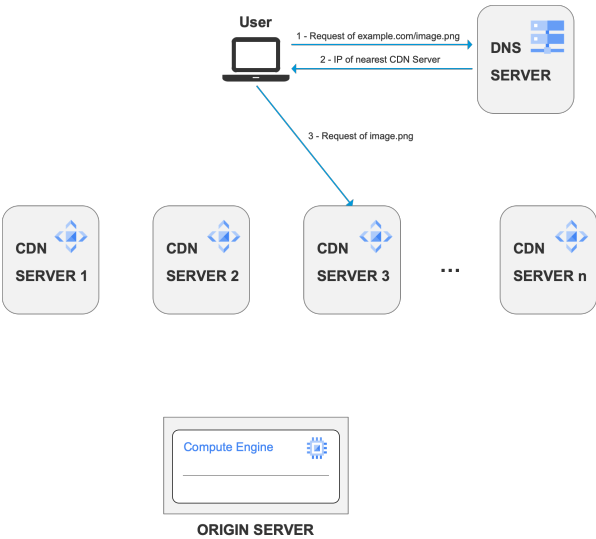
\includegraphics[keepaspectratio]{images/image71.png}}}

{I vantaggi portati dalle CDN sono:}

\begin{itemize}
\tightlist
\item
  {Velocità}
\item
  {Scalabilità}
\item
  {Protezione DDoS}
\item
  {Monitoraggio traffico}
\item
  {Costi ridotti}
\end{itemize}

{}

\subsection{\texorpdfstring{{Google Cloud
CDN}}{Google Cloud CDN}}\label{h.ff77kcxh75jb}

{Sistema usato globalmente con EDGE POP per avere dati sempre vicino
agli utenti, abbinato ad un load balancer per avere un unico IP.}

{\pandocbounded{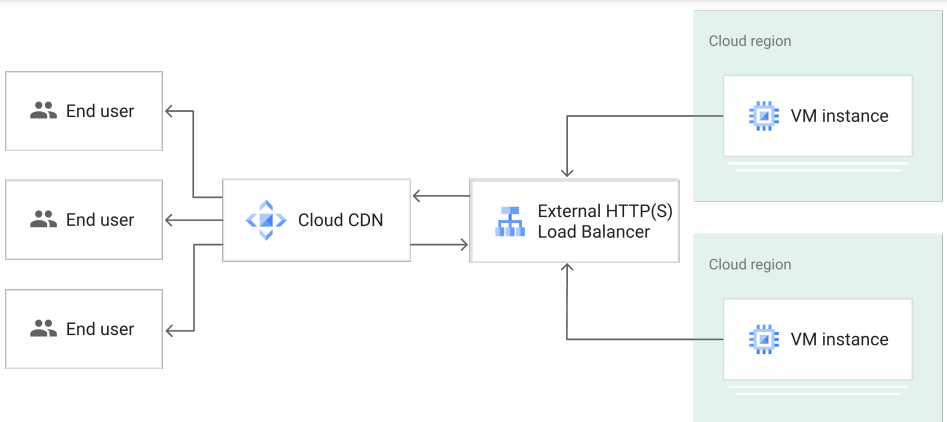
\includegraphics[keepaspectratio]{images/image70.png}}}

{Cloud CDN prevede tre modalità di gestione della cache: }

\begin{itemize}
\tightlist
\item
  {USE\_ORIGIN\_HEADERS}{:}{~Vengono usati appositi header, presenti
  nelle richieste dei dati, per determinare cosa inserire in cache e
  cosa no. }
\end{itemize}

{}

\begin{itemize}
\tightlist
\item
  {CACHE\_ALL\_STATIC}{: In automatico inserisce in cache tutti i dati
  statici, ovvero tutti i dati in cui è assente la direttiva no-store o
  no-cache. }
\end{itemize}

{}

\begin{itemize}
\tightlist
\item
  {FORCE\_CACHE\_ALL}{:}{~Vengono inserite in cache tutte le risposte,
  indipendentemente dagli header presenti}
\end{itemize}

{}

{}

{Infrastructure as Code (IaC)}

{}

{Invece di creare infrastrutture cloud manualmente si usa il codice, IaC
permette:}

\begin{itemize}
\tightlist
\item
  {creazione, gestione, rimozione di infrastrutture}
\item
  {integrazione con Continuos Integration}
\item
  {centralizzare la definizione dell\textquotesingle infrastruttura con
  anche il versioning}
\end{itemize}

{}

{Gli strumenti IaC sono Configuration o Provisioning.}

{}

\section{\texorpdfstring{{Configuration
tools}}{Configuration tools}}\label{h.kmluy5bzgox}

{Gestiscono la configurazione di infrastrutture già esistenti,
definendone uno stato di arrivo e gestendo le operazioni necessarie ad
ottenerlo.}

{}

{Implementati tramite linguaggi imperativi (definiscono le istruzioni da
eseguire per ottenere uno stato finale) e per questo sono non
idempotenti (due esecuzioni consecutive dello stesso codice possono
portare a risultati diversi ed inconsistenti) e non tengono conto dello
stato dell'infrastruttura tra un'esecuzione e l'altra.}

{}

\section{\texorpdfstring{{Provisioning
tools}}{Provisioning tools}}\label{h.sd2op287qe8c}

{Definiscono le operazioni necessarie alla creazione di nuove risorse
infrastrutturali in maniera veloce e consistente}

{}

{Implementati tramite linguaggi dichiarativi (descrivono il risultato
finale desiderato senza specificare i passi necessari per raggiungerlo)
quindi il codice è una rappresentazione diretta dello stato attuale
dell'infrastruttura, sono idempotenti (molteplici esecuzioni dello
stesso codice portano sempre allo stesso risultato).}

{}

{Fra i vantaggi abbiamo:}

\begin{itemize}
\tightlist
\item
  {Version control}
\item
  {Riuso}
\item
  {Modularità}{: possibilità di divisione del codice in diversi file con
  anche microservizi}
\item
  {Minori Errori}
\end{itemize}

{}

\section{\texorpdfstring{{Terraform}}{Terraform}}\label{h.belhetsjhnb3}

{Tool IoC, idempotente, open source, platform-agnostic (utilizzato su
molteplici cloud provider), per il provisioning dichiarativo di
infrastrutture cloud.}

{Sia Agentless che Masterless, quindi nessuna installazione nelle
risorse cloud.}

{}

{Si ua HLC
(}{\href{https://www.google.com/url?q=https://virtuale.unibo.it/pluginfile.php/2028975/mod_resource/content/1/Lezione\%25205\%2520-\%2520Infrastructure\%2520as\%2520Code.pdf&sa=D&source=editors&ust=1734628634294775&usg=AOvVaw3N0g6IboPdNRCqsK_AiRwk}{QUI}}{~da
slide 28 a 50}{) ~come linguaggio (dichiarativo) per i file di
configurazione che descrivono a Terraform le risorse necessarie per
realizzare una singola applicazione o l\textquotesingle intera
architettura; che poi genera un piano di esecuzione che descrive le
azioni da eseguire per raggiungere lo stato desiderato partendo dallo
stato attuale. Deploy nel dettaglio:}

{\pandocbounded{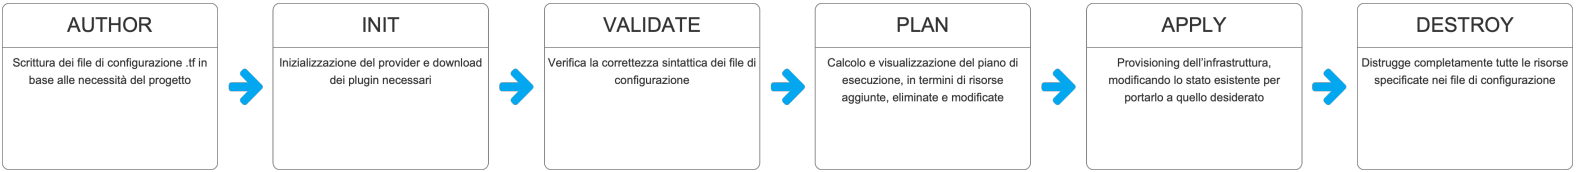
\includegraphics[keepaspectratio]{images/image62.png}}}

{}

{Le versioni sono:}

{\pandocbounded{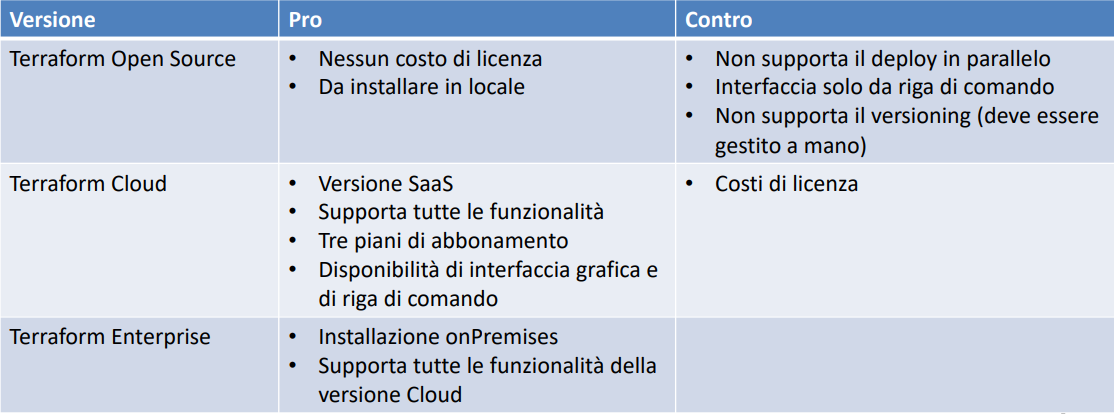
\includegraphics[keepaspectratio]{images/image22.png}}}

{Terraform mantiene uno "stato" dell\textquotesingle infrastruttura e
delle configurazioni previste, permette a terraform di mantenere le
corrispondenze tra le risorse create nell\textquotesingle infrastruttura
cloud e la loro definizione nei file tf.}

{La consistenza dello stato può diventare un problema quando più utenti
lavorano contemporaneamente alla definizione
dell\textquotesingle infrastruttura.}

{}

{Architetture moderne}

{Normalmente l'approccio che si usa per creare applicazioni è di tipo
}{monolitico}{, dove tutte le funzionalità sono nella stessa
}{code}{base. Questo rende l'applicazione architetturalmente semplice
migliorando la comunicazione fra i moduli e la scalabilità verticale.}

{Questo approccio porta svantaggi durante l'aggiornamento o la modifica
dell'applicazione con una complessità di gestione non indifferente.}

{}

{In sostanza è un approccio per progetti piccoli o legacy aumentando la
semplicità di sviluppo e di deploy.}

{}

\section{\texorpdfstring{{SOA}}{SOA}}\label{h.ejnuehns6ad8}

{Service Oriented Architecture, al contrario dell'approccio monolitico
lo scopo qui è dividere il più possibile in }{servizi }{sempre più
piccoli con specifici compiti che comunicando insieme formano un
applicazione e andando a scalare senza problemi in entrambi i sensi.}

{}

{I servizi sono fatti per essere il più autonomi possibili
(sviluppati/aggiornati in maniera separata), garantendo modularità
(unione di più servizi come si vuole per creare funzionalità),
astrazione e riusabilità.}

{}

\subsection{\texorpdfstring{{Architettura}}{Architettura}}\label{h.j85oof4qvn34}

{\pandocbounded{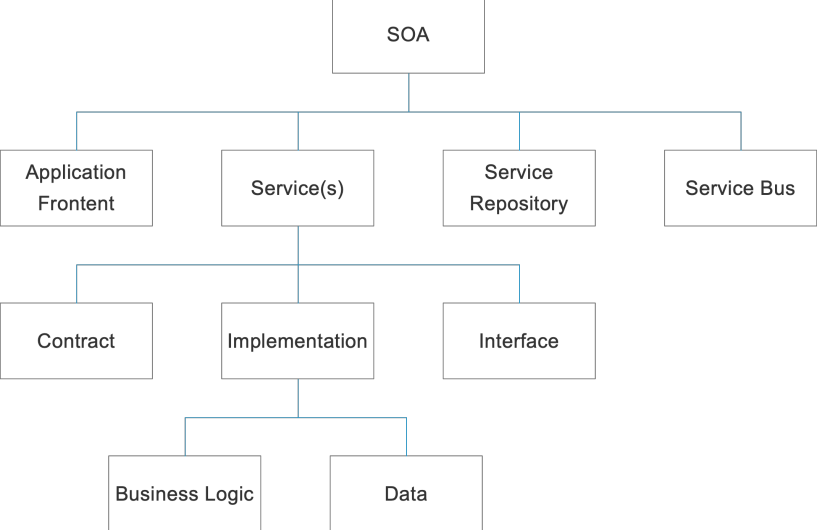
\includegraphics[keepaspectratio]{images/image30.png}}}

{}

{I vari componenti della SOA sono:}

\begin{itemize}
\tightlist
\item
  {Service}{: fulcro dell\textquotesingle architettura, coloro che
  implementano le funzionalità, composti da:}
\end{itemize}

\begin{itemize}
\tightlist
\item
  {Contract}{: definisce i dettagli tecnici e funzionali del servizio}
\item
  {Implementation}{: codice che implementa il contract}
\item
  {Interface}{: ~punto d' accesso al servizio}
\end{itemize}

\begin{itemize}
\tightlist
\item
  {Service Repository}{: archivio centralizzato con le informazioni di
  tutti i servizi disponibili nell\textquotesingle architettura }
\end{itemize}

{}

\begin{itemize}
\tightlist
\item
  {Application }{Frontend}{:}{~applicazione finale che utilizza i
  servizi}
\end{itemize}

{}

\begin{itemize}
\tightlist
\item
  {Service Bus}{: middleware per la comunicazione tra servizi,
  funzionalità:}
\end{itemize}

\begin{itemize}
\tightlist
\item
  {Mediazione}{: comunicazione senza la consapevolezza di
  }{quanti}{~servizi ci sono.}
\item
  {Routing dei messaggi}{: instradamento di messaggi dai servizi
  mittenti ai servizi destinatari in base alle regole di routing.}
\item
  {Trasformazione dei messaggi}{: trasformazione dei messaggi da un
  formato a un altro.}
\item
  {Gestione delle transazioni}{: coordinazione ~delle operazioni di più
  servizi.}
\item
  {Gestione degli errori e del monitoraggio: }{fornisce funzionalità per
  il monitoraggio dei servizi e per la gestione degli errori (gestione
  delle cose, ripristino operazioni fallite, registrazione eventi,
  ecc).}
\end{itemize}

{}

{Per comunicare, due servizi, devono seguire 4 fasi:}

\begin{enumerate}
\tightlist
\item
  {Il mittente (Service Consumer) contatta il Service Bus utilizzando il
  proprio formato di richiesta}
\item
  {Il Service Bus controlla il Service Registry per determinare il
  formato di richiesta accettato dal destinatario. Se necessario
  effettua la traduzione}
\item
  {Il Service Bus contatta il destinatario (Service Producer) usando il
  formato da esso richiesto}
\item
  {Il Service producer risponde utilizzando il proprio formato, che sarà
  tradotto dal service bus prima di inviarlo al service consumer}
\end{enumerate}

{}

\subsection{\texorpdfstring{{SOAP}}{SOAP}}\label{h.jmhnvydlh3yl}

{~O Simple Object Access Protocol, è un protocollo che indica il formato
standard per la comunicazione tra servizi web. Usato per evitare al
Service Bus di effettuare traduzioni.}

{}

{Il messaggio è formato dalle Envelope che }{contiene}{~l'header (info
del messaggio come mittente e destinatario) e il body (messaggio vero e
proprio) della richiesta.}

{}

\subsection{\texorpdfstring{{WSDL}}{WSDL}}\label{h.l4dtyg6mts0a}

{O Web Services Definition Language, un linguaggio di descrizione di
servizi utilizzato per definire l\textquotesingle interfaccia in modo
standardizzato e indipendente dal linguaggio di programmazione.}

{}

\section{\texorpdfstring{{Microservizi}}{Microservizi}}\label{h.bpjx6fssz0mt}

{L'evoluzione di SOA per tutte quelle aziende che devono muoversi in
maniera rapida per adattarsi in fretta ai cambiamenti del mercato e non
possono permettersi di seguire un modello ancora troppo centralizzato ed
articolato.}

{}

{Per questo è nato un pattern architetturale che struttura
un'applicazione come un insieme di microservizi indipendenti,
completamente decentralizzati e pensati come una istanza applicativa.
Favorevole alla virtualizzazione, al cloud e ai IaC e che tramite un
approccio metodologico chiamato}{~Agile Movement}{~consente di
sviluppare più rapidamente un software e le sue funzionalità.}

{\pandocbounded{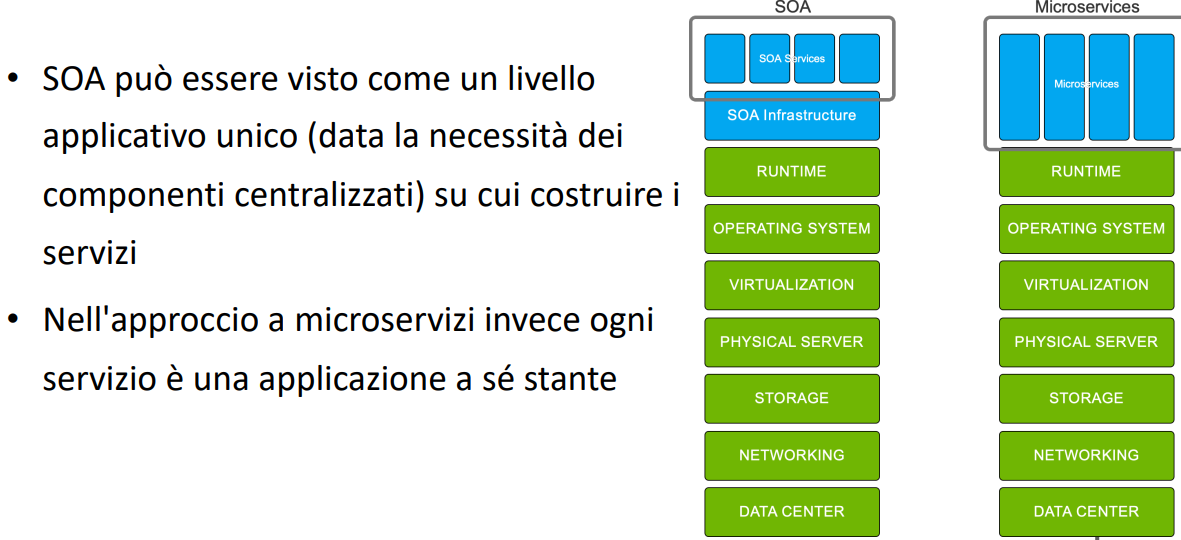
\includegraphics[keepaspectratio]{images/image45.png}}}

{Inoltre il DB, al contrario del SOA, è diviso per ogni micro servizio
che ne ha uno proprio.}

{}

{Ovviamente anche i microservizi hanno svantaggi, soprattutto se si
viene dal mondo SOA, infatti si ha un }{cambiamento significativo}{~nel
progettare app. Per non parlare della }{complessità }{dell'architettura
sottostante che porta i temi di load balancing, sicurezza e monitoraggio
a tener conto di molteplici elementi.}

{}

\subsection{\texorpdfstring{{REST}}{REST}}\label{h.vv23bqa3grjd}

{Soluzione alternativa a SOAP per i microservizi, basato sul protocollo
HTTP quindi:}

\begin{itemize}
\tightlist
\item
  {Orientato alle risorse}{: i microservizi espongono risorse
  accessibili tramite REST (identificate da URI).}
\end{itemize}

{}

\begin{itemize}
\tightlist
\item
  {Client server e request-response}{: il server aspetta le richieste (i
  vari verbi HTTP come GET , POST, ecc) e successivamente risponde solo
  se arrivano.}
\end{itemize}

{}

\begin{itemize}
\tightlist
\item
  {Stateless}{: il server non ha stati applicativi.}
\end{itemize}

{}

{I microservizi espongono la propria interfaccia API per richiedere le
risorse e per questo i servizi sono }{Restful API}{. Le API sono nella
forma classica; Esempio:}

{\pandocbounded{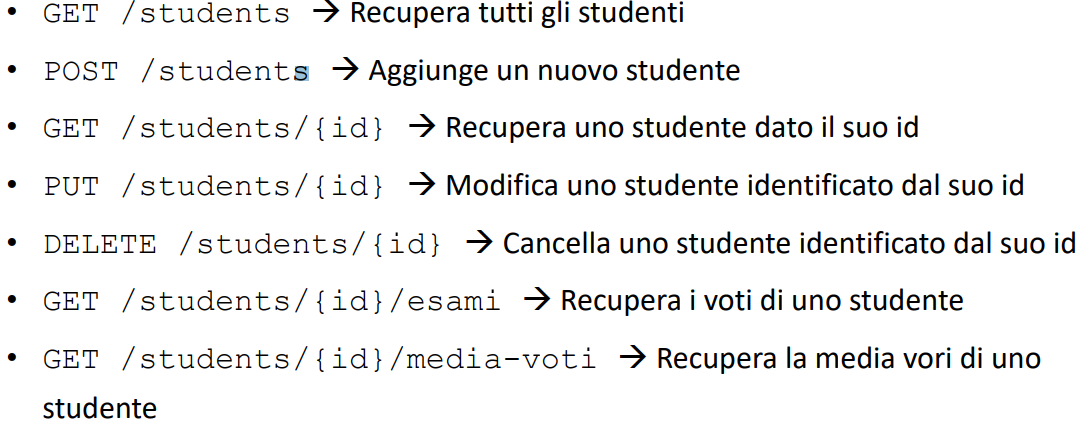
\includegraphics[keepaspectratio]{images/image60.png}}}

{Questo modo rende la piattaforma e il linguaggio indipendente con una
semplicità e flessibilità unica. Ed essendo stateless la scalabilità
orizzontale è possibile sui microservizi.}

{}

{Il formato dei messaggi è il JSON
(}{\href{https://www.google.com/url?q=https://virtuale.unibo.it/pluginfile.php/2036712/mod_resource/content/1/Lezione\%25206\%2520-\%2520Architetture\%2520Moderne.pdf&sa=D&source=editors&ust=1734628634303331&usg=AOvVaw1-ewv6x-KhdYRylZ8dNy86}{QUI}}{~da
slide 46 a 50).}

{}

\section{\texorpdfstring{{Event Driven
Architecture}}{Event Driven Architecture}}\label{h.yew98yfrjmjl}

{O EDA, è un pattern che si basa sulla comunicazione asincrona basata su
eventi tra sistemi tramite rapporto publisher/subscriber. Usata in
applicazioni IoT o messaggistica.}

{}

{In sostanza il }{publisher }{è un sistema che pubblica un evento in
determinate condizioni e il sistema }{subscriber }{si registra a
quell\textquotesingle evento ricevendo una notifica/messaggio quando le
condizioni sono verificate.}

{Per funzionare c'è bisogno di un }{Event}{~Broker }{che gestisce le
pubblicazioni, le sottoscrizioni e le notifiche.}

{}

{i vantaggi sono:}

\begin{itemize}
\tightlist
\item
  {Indipendenza}{~tra servizi.}
\item
  {Scalabilità.}
\item
  {Real-time}{~grazie all'alto grado di parallelismo si possono gestire
  grandi volumi di messaggi e flussi dati.}
\end{itemize}

{}

\subsection{\texorpdfstring{{Pub / Sub
model}}{Pub / Sub model}}\label{h.aism9vq36sen}

{\pandocbounded{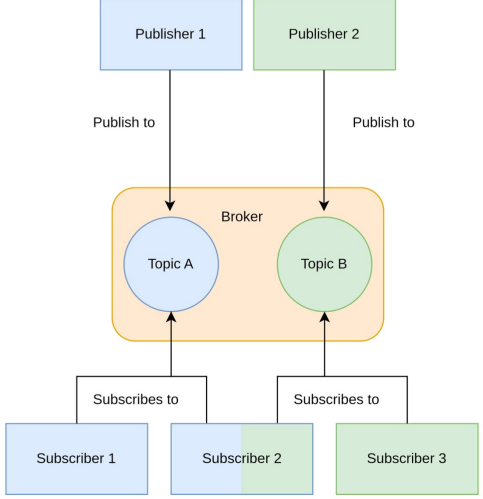
\includegraphics[keepaspectratio]{images/image15.png}}}

{Nel dettaglio:}

{\pandocbounded{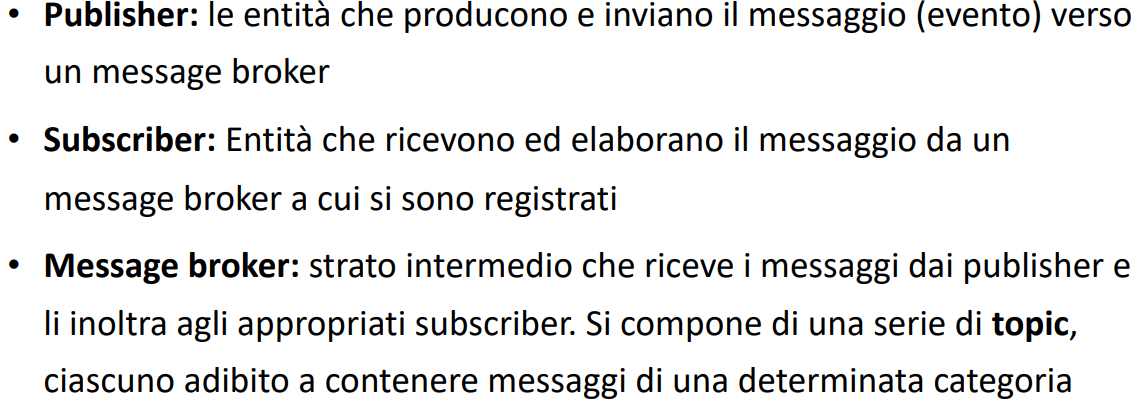
\includegraphics[keepaspectratio]{images/image20.png}}}

{}

{I sub si possono iscrivere a uno o più topic e quando il pub manda
l\textquotesingle evento al topic il broker lo riceve e lo archivia.
SUccessivamente tramite broker si può fare }{Push}{~(inoltro ai sub) o
}{Pull}{~(i sub verificano da soli i messaggi).}

{}

{Containers}

{Per risolvere le criticità che i microservizi portano alle
applicazioni, come l'impossibilità di isolare i microservizi iper
aggiornamenti o non poterli trasferire da un SO ad un altro, sono nati i
container.}

{}

{Tecnologia di virtualizzazione senza hypervisor (a livello SO) dove
ogni container è un pacchetto di applicazioni con relative dipendenze
che condividono fra loro solo il kernel linux del SO host, completamente
indipendenti in termini di file system, processi, memoria e networking.}

{\pandocbounded{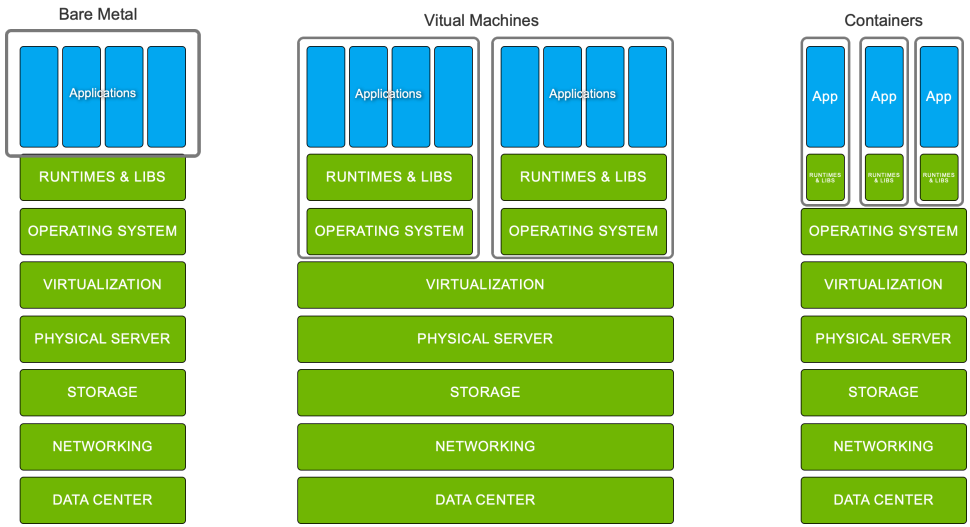
\includegraphics[keepaspectratio]{images/image32.png}}}

{}

{Rispetto alle VM i container hanno migliori performance, meno
dipendenze con il SO e virtualizzazione innestata cioè VM con dentro
containers:}

{\pandocbounded{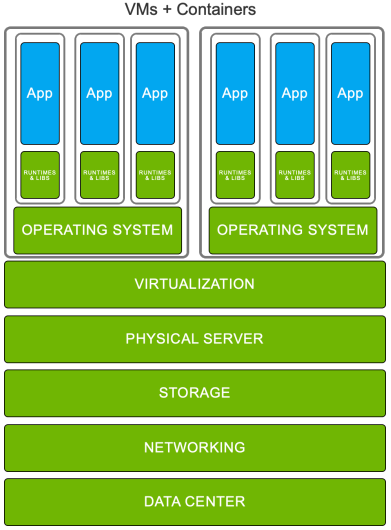
\includegraphics[keepaspectratio]{images/image4.png}}}

{L\textquotesingle isolamento è reso possibile dal LinuX Container (LXC)
composto da due tecnologie, Cgroups e Namespaces, che ora vediamo.}

{}

\subsection{\texorpdfstring{{Control
Groups}}{Control Groups}}\label{h.v7elc05aqig3}

{O cgroups, utilizzato dal kernel linux per la gestione dell'utilizzo
delle risorse da un insieme di processi specifici, organizzati in
maniera gerarchica con struttura ad albero con ogni nodo che è un gruppo
con certe regole.}

{}

\subsection{\texorpdfstring{{Namespaces}}{Namespaces}}\label{h.mgstqenqk0uu}

{Il kernel Linux lo usa per creare risorse virtuali, come
}{astrazione}{~di risorse fisiche, che sostanzialmente dice ad un
determinato processo di usare solamente le risorse assegnate al suo
stesso namespace.}

{}

\subsection{\texorpdfstring{{S.O.}}{S.O.}}\label{h.noigqxjshplb}

{I container non possono eseguire }{SO differenti}{~a Linux, ma possono
decidere quale distribuzione usare, anche se differente a quella
dell'host.}

{}

{Come già si sarà intuito l'unico modo per usare i container su Windows
è farlo con una VM Linux, quindi impossibile farlo in maniera nativa.}

{}

\section{\texorpdfstring{{Docker}}{Docker}}\label{h.5pno6qnv7h2m}

{Sistema di virtualizzazione open source e client server basato su
container, composto da:}

\begin{itemize}
\tightlist
\item
  {Docker Daemon}{: il processo responsabile della gestione di immagini
  e container }
\item
  {Docker Client}{: l\textquotesingle applicazione con cui fornire
  comandi al daemon }
\item
  {Docker Registry}{: Il repository delle immagini}
\end{itemize}

{\pandocbounded{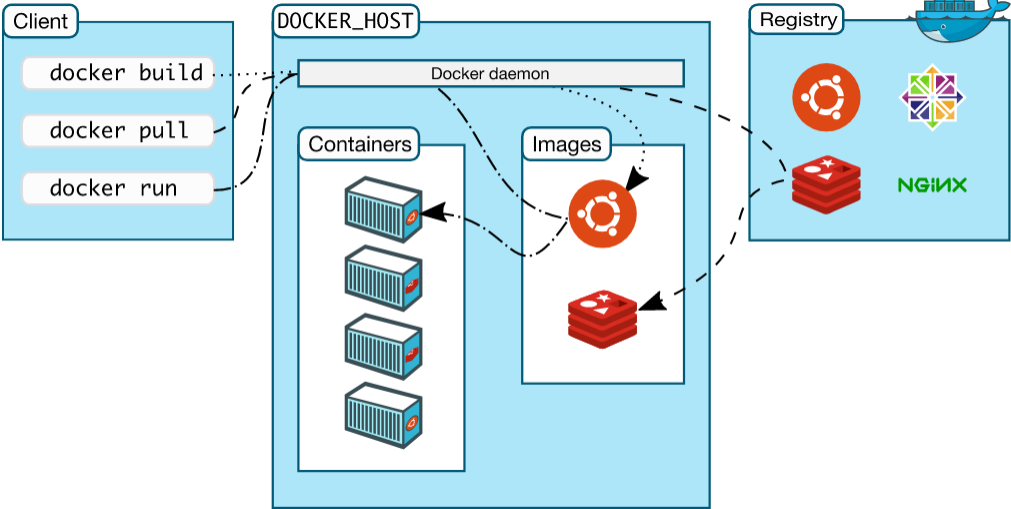
\includegraphics[keepaspectratio]{images/image13.png}}}

{\pandocbounded{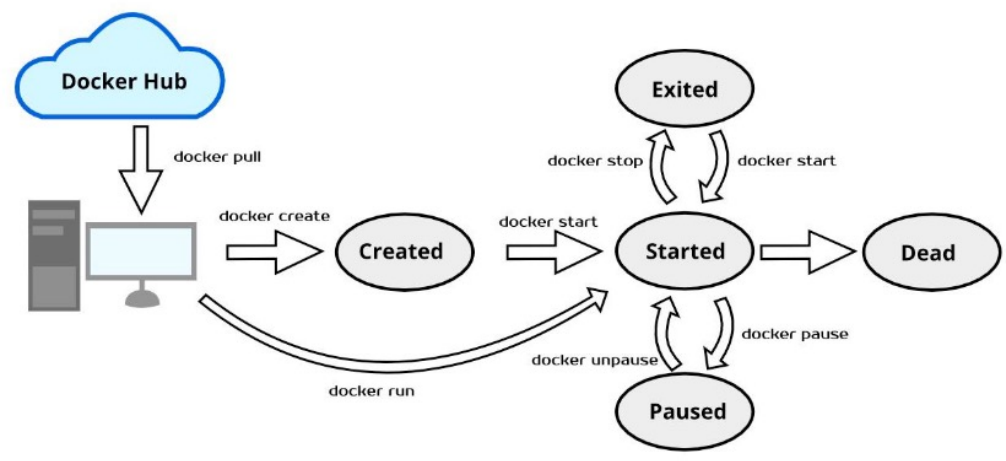
\includegraphics[keepaspectratio]{images/image66.png}}}

{ciclo di vita}

{}

{Docker si basa sul concetto di immagini, template in sola lettura dai
quali derivare i container che verranno messi in esecuzione.}

{Il rapporto tra immagine e container può essere paragonato al rapporto
tra classe e oggetto esistente nei linguaggi di programmazione
(}{container è una istanza di una immagine}{)}

{}

\subsection{\texorpdfstring{{Immagini}}{Immagini}}\label{h.66142ewwvybi}

{Versione immutabile, in sola lettura e strutturata in layer ordinati di
un software, salvati in questo modo:}

{}

{host/registry/image:tag}

{}

{Dove:}

\begin{itemize}
\tightlist
\item
  {Host}{: Il nome del server in cui è memorizzata
  l\textquotesingle immagine }{(p.e.}{~docker.io) }
\item
  {Registry}{: Il nome del repository in cui è contenuta
  l\textquotesingle immagine }
\item
  {Image}{: Il nome dell\textquotesingle immagine }
\item
  {Tag}{: L\textquotesingle identificativo della versione
  dell\textquotesingle immagine, scelto in modo arbitrario, quello di
  default è }{latest}{.}
\end{itemize}

{}

{Ogni layer definisce un aspetto di quello che sarà il filesystem finale
dell\textquotesingle immagine e in fase di creazione sono "eseguiti" in
sequenza, dando origine al file system definitivo.}

{Anch\textquotesingle essi sono immutabili permettendo la condivisione
tra immagini.}

\subsubsection{\texorpdfstring{{Docker
File}}{Docker File}}\label{h.s0tfc13b76ng}

{File che definisce come i layer compongono un'immagine, dove ad ogni
riga equivale ad un layer:}

{\pandocbounded{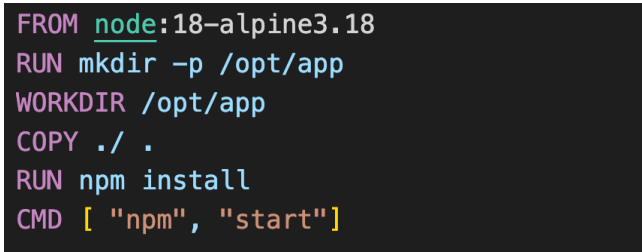
\includegraphics[keepaspectratio]{images/image38.png}}}

{}

\subsection{\texorpdfstring{{Container}}{Container}}\label{h.vndwg8cz8s1n}

{La creazione di un container aggiunge un ulteriore layer a quelli
presenti nell\textquotesingle immagine di partenza, collocato sopra a
tutti gli altri (eseguito per ultimo) e non condivisibile.}

{Questo layer permette ai container di effettuare modifiche al file
system in modo indipendente dagli altri container nati dalla stessa
immagine.}

{}

\subsection{\texorpdfstring{{Docker
Hub}}{Docker Hub}}\label{h.55zqjvvem37h}

{Repo gestito direttamente da docker per la condivisione di immagini}

{}

\subsection{\texorpdfstring{{Artifact
Registry}}{Artifact Registry}}\label{h.akw1bobn7wur}

{Repo gestito direttamente da Google per la condivisione di immagini
(non solo docker)}

{}

\section{\texorpdfstring{{Google Cloud
Run}}{Google Cloud Run}}\label{h.d00k5iodawqx}

{Servizio PaaS per l\textquotesingle esecuzione di docker container
completamente gestito da Google, fatturato solo il tempo di utilizzo,
calcolato al decimo di secondo.}

{}

{Cloud Run genera un url pubblico (in https) con cui accedere
direttamente al container, deploy configurato in termini di: }

\begin{itemize}
\tightlist
\item
  {Variabili d\textquotesingle ambiente }
\item
  {Modalità di accesso (autenticata / non autenticata) }
\item
  {Networking (gestione del traffico in entrata e in uscita) }
\end{itemize}

{}

{Cloud run inoltre gestisce l\textquotesingle aggiornamento del
container, in modo che questo possa avvenire senza interrompere il
servizio.}

{}

\section{\texorpdfstring{{Kubernetes}}{Kubernetes}}\label{h.ydx7f3krmfly}

{}

\subsection{\texorpdfstring{{Container
Orchestration}}{Container Orchestration}}\label{h.ib0qzz7bkcw}

{Su Docker la gestione può diventare estremamente complessa in scenari
altamente strutturati, per questo sarebbe utile disporre di
Orchestratori di Container, ovvero applicazioni in grado di gestire
tutti gli aspetti legati all\textquotesingle utilizzo combinato di più
container.}

{\pandocbounded{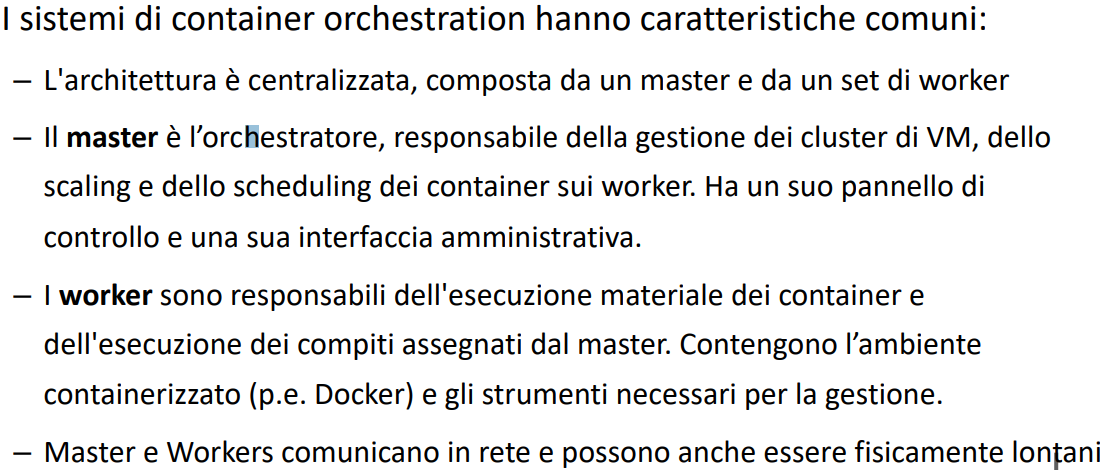
\includegraphics[keepaspectratio]{images/image10.png}}}

{}

\subsection{\texorpdfstring{{Kubernetes}}{Kubernetes}}\label{h.n17tb5svqbuf}

{Nato per permettere ai container di sfruttare le potenzialità
dell\textquotesingle infrastruttura cloud, superando i limiti di Docker
nel coordinare progetti complessi con la possibilità di automatizzare il
deploy, la scalabilità e le operazioni di gestione di applicazioni
}{conteinerizzate}{~su gruppi di host (istanze VM).}

{}

{Architettura Master/Worker, con cluster composti da nodi dove uno
specifico è il master con funzionalità diverse dai worker.}

{\pandocbounded{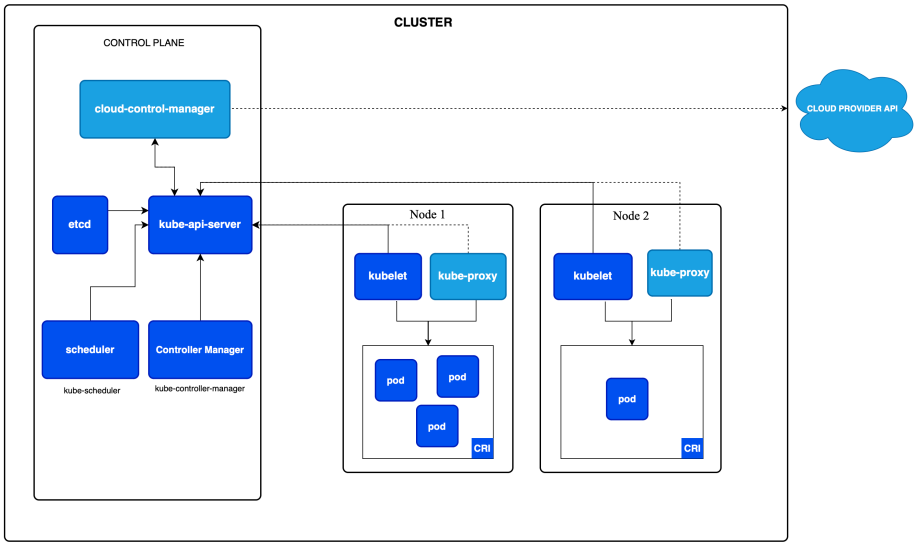
\includegraphics[keepaspectratio]{images/image9.png}}}

{}

{i componenti worker sono:}

\begin{itemize}
\tightlist
\item
  {Pod}{: è la più piccola unità che può essere creata e gestita in
  Kubernetes. I pod contengono i container da eseguire (approfondiremo
  tra poco) }
\end{itemize}

{}

\begin{itemize}
\tightlist
\item
  {Kubelet}{:}{~Servizio che gestisce i pod e le risorse da essi
  utilizzate (container, immagini, volumi\ldots) }
\end{itemize}

{}

\begin{itemize}
\tightlist
\item
  {Kube-proxy}{: Servizio di proxy che opera anche da load balancer per
  inoltrare il traffico verso il pod appropriato.}
\end{itemize}

{}

{I componenti master sono:}

\begin{itemize}
\tightlist
\item
  {Scheduler}{: Determina su quale nodo deve essere eseguito un Pod }
\end{itemize}

{}

\begin{itemize}
\tightlist
\item
  {Ap}{i }{Server}{: È l\textquotesingle interfaccia REST per interagire
  con il master }
\end{itemize}

{}

\begin{itemize}
\tightlist
\item
  {Controller Manager}{: Responsabile dei controlli di replicazione e
  delle relative azioni}
\end{itemize}

{}

\begin{itemize}
\tightlist
\item
  {Etcd}{: Database key/value usato dal Master per memorizzare tutte le
  informazioni persistenti di cui ha bisogno}
\end{itemize}

{}

\subsection{\texorpdfstring{{Pods}}{Pods}}\label{h.jco7y64z5kiw}

{Unità più piccola gestita, insieme di container raggruppati logicamente
per poter lavorare insieme. I container dei pod possono essere visti
come processi di una VM (dove la VM è il pod) che comunicano fra loro
condividendo IP e porta e volumi condivisi (come dischi di una VM).}

{}

{Hanno un ciclo di vita corto, si creano, si assegna un ID e vengono
schedulati sui nodi.}

\subsubsection{\texorpdfstring{{Deployment \&
Replicasets}}{Deployment \& Replicasets}}\label{h.x16bhexfu47a}

{Strumenti per la replicazione di pod, il primo lavora ad un livello più
alto del secondo.}

{}

{Il deployment è un insieme di Pod identici definiti tramite yaml, il
suo scopo è specificare il numero di repliche che dovranno essere
eseguite, se alcune falliscono le riattiva finché non si torna a quel
determinato numero, e applicare ogni modifica fatta al template yaml
ricreando i pod con strategie di aggiornamento.}

{}

{Un }{ReplicaSets}{~funziona come un deployment (garantisce che un certo
numero di pods in ogni istante di tempo), solo che non gestisce
strategie di aggiornamento.}

{}

\subsection{\texorpdfstring{{Services}}{Services}}\label{h.3pvs122m9h34}

{~I servizi sono un insieme di pod indipendenti affiancati da modalità
d'accesso, raggruppati tramite selettori, che assicura la possibilità di
raggiungere il pod appropriato senza preoccuparsi della posizione.}

{}

{Per farlo si usa un IP (o nome di dominio) che i consumatori useranno,
come questo servizi vengono esposti si creano alcuni tipi:}

\begin{itemize}
\tightlist
\item
  {ClusterIP}{: Espone il servizio sulla rete interna del cluster,
  }{rendendolo }{ina}{ccessibile}{~dall\textquotesingle esterno. È il
  default. }
\end{itemize}

{}

\begin{itemize}
\tightlist
\item
  {NodePort}{: Espone il servizio mappando un cluster ip su una porta di
  ogni nodo, rendendo il servizio è raggiungibile tramite
  l\textquotesingle ip di ogni nodo. }
\end{itemize}

{}

\begin{itemize}
\tightlist
\item
  {LoadBalancer}{: Espone il servizio su un indirizzo ip raggiungibile
  dall\textquotesingle esterno. Fa uso di NodePort (e quindi di
  ClusterIP)}
\end{itemize}

{}

\subsection{\texorpdfstring{{GKE - Google Kubernetes
Engine}}{GKE - Google Kubernetes Engine}}\label{h.oqhiclqcxiny}

{Servizio Google per creare/utilizzare cluster kubernetes, con gestione
di master e worker e funzionalità native per sfruttare al meglio
kubernetes tra cui load balancing, scaling automatico dei nodi,
monitoraggio delle risorse, patch di sicurezza ecc.}

{}

{}

{Devops}

\section{\texorpdfstring{{SDLC}}{SDLC}}\label{h.uj08a4a1ce59}

{Software Development Life Cycle, letteralmente il ciclo di vita del
software che parte dall'analisi e finisce con la pubblicazione e il
futuro mantenimento.}

{\pandocbounded{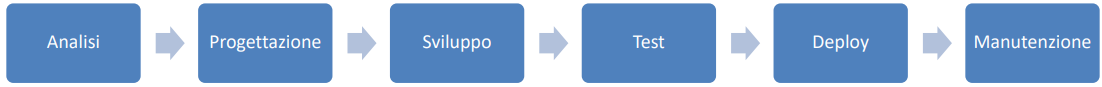
\includegraphics[keepaspectratio]{images/image43.png}}}

{}

\subsection{\texorpdfstring{{Analisi}}{Analisi}}\label{h.27u7twfa5lib}

{Raccolta dei requisiti funzionali e non funzionali tramite interviste,
sondaggi o osservazioni fatte alle persone rilevanti, i cosiddetti
stakeholder.}

{}

{Alla fine della raccolta si scrive tutto su un documento dove si
ordinano i requisiti in ordine di priorità.}

{}

\subsection{\texorpdfstring{{Progettazione}}{Progettazione}}\label{h.1wp42y42lw7v}

{Si progettano, in maniera coerente con il documento di analisi, le
varie parti architetturali dell'applicazione, ogni parte ha una tecnica
specifica:}

\begin{itemize}
\tightlist
\item
  {Struttura del codice}{~à pattern architetturali, diagrammi UML
  (class, sequence, activity diagrams) }
\item
  {Struttura dei database}{~à progettazione E/R }
\item
  {User Interface}{~à User experience design }
\item
  {Caratteristiche dei server o delle piattaforme cloud}{~à cloud
  engineering}
\end{itemize}

{}

\subsection{\texorpdfstring{{Sviluppo}}{Sviluppo}}\label{h.f2g4hiuuvqh7}

{Si inizia a scrivere il codice andando dietro a quello fatti nella fase
di progettazione, utilizzando versioneing e scrivendo i primi test.}

{}

\subsection{\texorpdfstring{{Test}}{Test}}\label{h.t5n6rgl4izvw}

{Si verifica che il codice sia conforme con tutti i requisiti
(funzionali e non) e a tutte le scelte progettuali, i test hanno diversi
livelli:}

\begin{itemize}
\tightlist
\item
  {Unit e Integration testing}{: Per verificare
  l\textquotesingle assenza di bug nel codice }
\item
  {System testing}{: Per verificare la presenza di tutte le feature
  richieste e la corrispondenza con le specifiche }
\item
  {Performance testing }
\item
  {Usability testing }
\item
  {Security testing}
\end{itemize}

{}

\subsection{\texorpdfstring{{Deploy}}{Deploy}}\label{h.muz2fwm9o659}

{Fase cruciale dove si rilascia il software, per farlo }{si
usano}{~diverse tattiche. Bisogna garantire continuità e rollback.}

\subsubsection{\texorpdfstring{{Complete
Deployment}}{Complete Deployment}}\label{h.3x3whslfcavb}

{O Big Bang Deployment, consiste nel fare deployment e rilascio di tutte
le componenti in una volta. }

{}

{Alto rischio, usata per architetture monolitiche, con poche opzioni di
ripristino se qualcosa va storto.}

{\pandocbounded{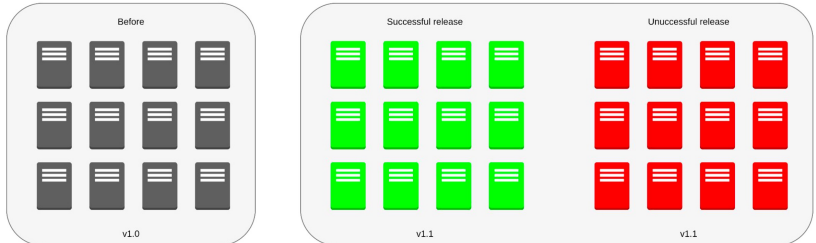
\includegraphics[keepaspectratio]{images/image23.png}}}

\subsubsection{\texorpdfstring{{Rolling
Deployment}}{Rolling Deployment}}\label{h.b6h3pdndqsk5}

{Fatto una componente alla volta, procedendo alla successiva se la
precedente funziona correttamente, minimizzando di parecchio il rischio
di fallimento completo.}

{\pandocbounded{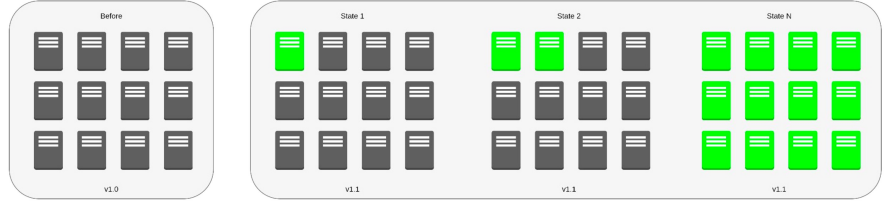
\includegraphics[keepaspectratio]{images/image61.png}}}

\subsubsection{\texorpdfstring{{Blue/Green
Deployment}}{Blue/Green Deployment}}\label{h.etzznr1zifwv}

{Vengono mantenute due copie identiche dell'infrastruttura,
}{denominandole blu}{~e verde. L\textquotesingle ambiente in uso dagli
utenti è quello blu, mentre gli aggiornamenti sono deployati sul verde.
Se quella verde ha problemi si fa il rollback sulla blu.}

{}

{Costosa ma efficace.}

{\pandocbounded{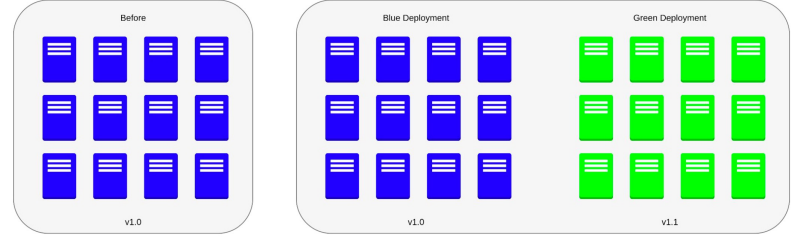
\includegraphics[keepaspectratio]{images/image39.png}}}

\subsubsection{\texorpdfstring{{Canary
Deployment}}{Canary Deployment}}\label{h.2fczwf3k0xp}

{Viene fatto il deployment e il rilascio della nuova versione solo ad
una piccola percentuale di utenti (casualmente scelti), si monitora
l'andamento fino al rilascio completo.}

{\pandocbounded{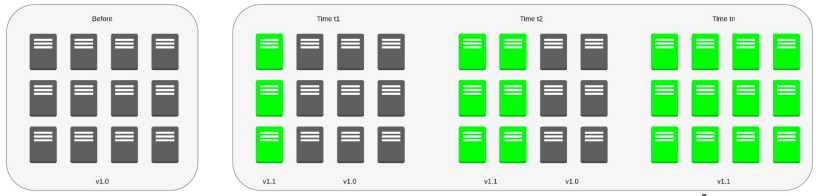
\includegraphics[keepaspectratio]{images/image64.png}}}

{}

\subsection{\texorpdfstring{{Manutenzione}}{Manutenzione}}\label{h.6zqlu5p7xdva}

{Si monitora il software per problemi e bug tramite sistemi di bug
tracking ed eventualmente risolti in base alla priorità.}

{}

\section{\texorpdfstring{{Metodologie}}{Metodologie}}\label{h.mutwff73swwj}

\subsection{\texorpdfstring{{Waterfall}}{Waterfall}}\label{h.wazpz9kp4s1r}

{Fasi eseguite in stretto ordine sequenziale. Si può procedere ad una
fase solo se la successiva è completamente terminata.}

{}

{Adatto per grandi progetti, ben strutturati, con requisiti chiari e ben
definiti.}

{\pandocbounded{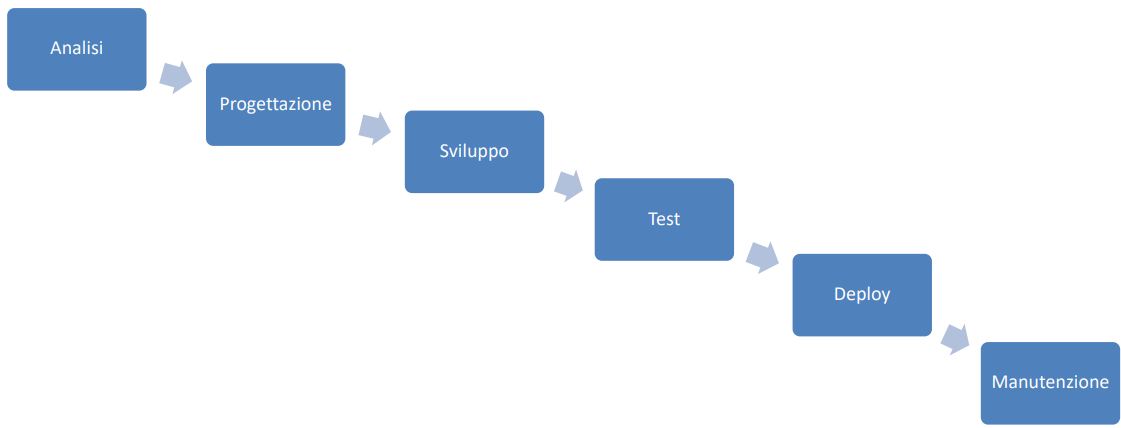
\includegraphics[keepaspectratio]{images/image50.png}}}

{}

\subsection{\texorpdfstring{{Agile}}{Agile}}\label{h.y4xqhmjsba1h}

{Ne esistono tante, ma tutte sono volte alla flessibilità con rilasci
intermedi del software, non complete ma funzionanti.}

{}

{Lo sviluppo procede pertanto con una sequenza di iterazioni dette
sprint, intervallati da incontri regolari (stand-up meetings) tra i
componenti del team per effettuare la pianificazione a breve termine e
per tenersi aggiornati sugli avanzamenti.}

{\pandocbounded{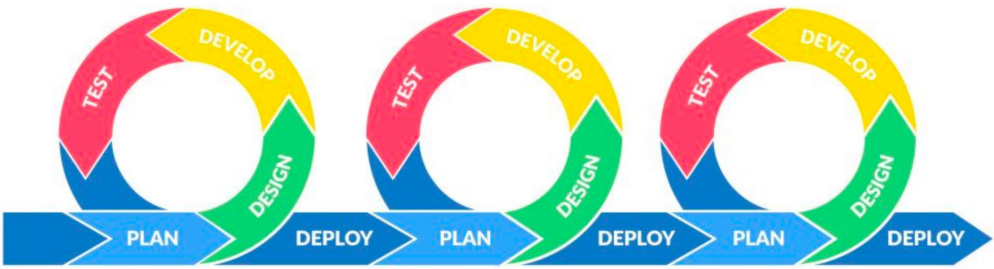
\includegraphics[keepaspectratio]{images/image49.png}}}

{}

\subsection{\texorpdfstring{{Devops}}{Devops}}\label{h.hgwim57qe2jk}

{Nata per favorire la comunicazione tra sviluppatori e reparto IT che
non accadeva dell'Agile (incentrate sulla comunicazione fra soli
sviluppatori).}

{}

{Crea pipeline per automatizzare task ripetitivi dal software
development al rilascio finale. Utilizza i microservizi incentivando la
sperimentazione.}

{\pandocbounded{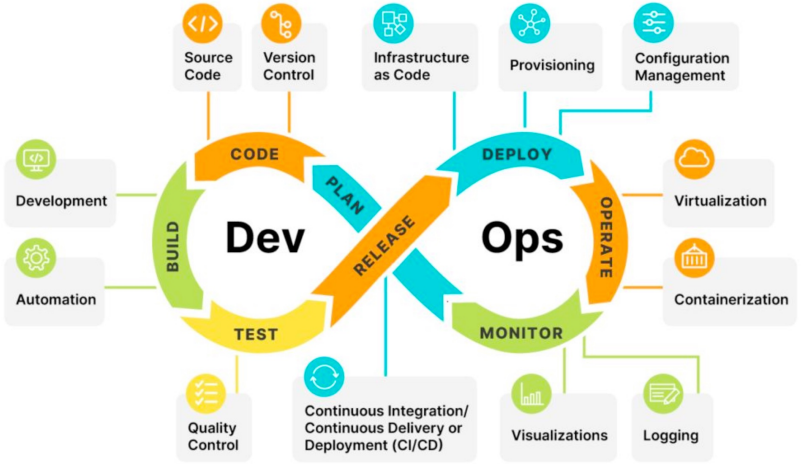
\includegraphics[keepaspectratio]{images/image35.png}}}

{}

{}

\section{\texorpdfstring{{CI/CD}}{CI/CD}}\label{h.b4xz4uw6nl8e}

{L'insieme di CI e CD riduce i rischi semplificando l'individuazione dei
bug e permettendo di ridurre al minimo il time to market}

\subsection{\texorpdfstring{{CI}}{CI}}\label{h.tp287horzrm7}

{La Continuous Integration (CI) è un processo che prevede di integrare
il codice degli sviluppatori in un repository condiviso, più volte al
giorno. Ogni check-in di codice è poi verificato tramite una build
automatica in modo da rilevare prima possibile eventuali problemi.}

{\pandocbounded{\includegraphics[keepaspectratio]{images/image52.png}}}

\subsection{\texorpdfstring{{CD}}{CD}}\label{h.cay273mjkdjj}

{Il Continuous Deployment (CD) è strettamente collegato al processo di
CI e si occupa di rilasciare in produzione il software che ha superato
le fasi del processo di integrazione; tramite strategie di deploy,
notifica e eventuali autorizzazioni manuali.}

{\pandocbounded{\includegraphics[keepaspectratio]{images/image56.png}}}

{}

\subsection{\texorpdfstring{{Su Google CLoud
Platform}}{Su Google CLoud Platform}}\label{h.j8l7n8z9co0g}

{GCP fornisce due strumenti di CI/CD: }

\begin{itemize}
\tightlist
\item
  {Cloud }{Build}{:}{~strumento di CI con alcune possibilità di
  deployment, elabora una repository applicandogli degli step di build
  riportati in un file YAML.}
\end{itemize}

{~}

\begin{itemize}
\tightlist
\item
  {Cloud Deploy:}{~strumenti di CD a partire da build già pronte,
  automatizza la distribuzione delle app su alcuni ambienti.}
\end{itemize}

{}

{Entrambi serverless ed è sufficiente }{configurarli}{~utilizzando un
file YAML.}

{}

{Monitoraggio e Logging}

\section{\texorpdfstring{{Logging}}{Logging}}\label{h.7rv8zgf87wux}

{Quando si registrano eventi e informazioni da un app/sistema per
estrarre informazioni sulle attività per comprendere meglio l'uso o
errori del sistema.}

{}

{I log si possono analizzare in real time o salvati in file di testo o
DB, infatti i log hanno una forma strutturata con timestamp e gravità, e
un contesto/contenuto chiaro e ben definito.}

{}

{Alcuni use case dei log potrebbero essere:}

\begin{itemize}
\tightlist
\item
  {Debug}
\item
  {Auditing}{: cioè registrare chi fa cosa.}
\item
  {Performance monitor}{: per identificare colli di bottiglia e degrado
  delle performance.}
\item
  {Trend Analysis}{: salvataggio di informazioni per creare serie
  temporali.}
\end{itemize}

{}

\subsection{\texorpdfstring{{Timestamp}}{Timestamp}}\label{h.xtvhfrd9fkma}

{Esatto momento in cui il logg si è generato, si usa l'orologio di
sistema per avere la data e l'ora precisa e per questo va sempre tenuto
sincronizzato.}

{}

{I due formalismi principali sono:}

\begin{itemize}
\tightlist
\item
  {~ISO 8601 → ~2024-04-23T14:16:49.272Z}{. Dove T separa data e ora e Z
  indica che il tempo è riferito al fuso orario di Greenwich.}
\end{itemize}

{}

\begin{itemize}
\tightlist
\item
  {Unix Time → 1713881809}{. Tempo espresso in numero di secondi
  trascorsi dal 1 gennaio 1970.}
\end{itemize}

{}

\subsection{\texorpdfstring{{Severity}}{Severity}}\label{h.b0vfgaz3k55f}

{La gravità serve per dare priorità ad eventi gravi ed effettuare
analisi e filtraggio una scala potrebbe essere:}

{\pandocbounded{\includegraphics[keepaspectratio]{images/image7.png}}}

{}

\subsection{\texorpdfstring{{Strumenti}}{Strumenti}}\label{h.ft1edahcsrwc}

{Alcuni strumenti per gestire, aggregare e analizzare i log possono
essere:}

\begin{itemize}
\tightlist
\item
  {ELK Stack}{: composto da tre prodotti. Un motore di ricerca
  (Elasticsearch), un gestore di log (Logstash) e un frontend di
  visualizzazione (Kibana) }
\end{itemize}

{}

\begin{itemize}
\tightlist
\item
  {Splunk}{: soluzione all-in-one che indicizza e processa i dati
  ricevuti per visualizzarli tramite avanzate modalità di ricerca (anche
  uso di ML per individuare anomalie)}
\end{itemize}

{}

{Entrambi i prodotti possono essere installati on-premises o su cloud
provider. Sono inoltre disponibili come SaaS.}

{}

\subsection{\texorpdfstring{{GCP Cloud
Logging}}{GCP Cloud Logging}}\label{h.zbqe733kxjd5}

{Servizio completamente gestito di gestione dei log, compatibile "out of
the box" con tutti i servizi GCP; può raccogliere, memorizzare, filtrare
e visualizzare i log raccolti dalla Cloud Logging API e consegnati ad
una destinazione (sink)}

{}

{I sink possono essere di tre tipi:}

\begin{itemize}
\tightlist
\item
  {Required log sink}{: Per memorizzare attività amministrative ed
  eventi di sistema. Gli eventi sono memorizzati per 400 giorni e non
  c\textquotesingle è possibilità di modifica.}
\end{itemize}

{}

\begin{itemize}
\tightlist
\item
  {Default log sink}{: Per tutti gli eventi che non sono inviati al
  required sink. La retention di default è di 30 giorni ma può essere
  modificata.}
\end{itemize}

{}

{I log possono essere esportati dall\textquotesingle archivio centrale
verso altre tipologie di storage, più adatte alle specifiche esigenze: }

\begin{itemize}
\tightlist
\item
  {Cloud Storage}{: per retention a lungo termine, risparmiando sui
  costi }
\end{itemize}

{}

\begin{itemize}
\tightlist
\item
  {BigQuery}{: per analisi approfondite, per correlazioni e per
  identificazione dei trend}
\end{itemize}

{}

\begin{itemize}
\tightlist
\item
  {Pub/Sub}{: per inviarli a strumenti di terze parti, registrati come
  subscriber di determinati topic}
\end{itemize}

{}

\section{\texorpdfstring{{Monitoring}}{Monitoring}}\label{h.mtvidbumm36y}

{Processo di raccolta ed osservazione di dati operativi e di performance
dei sistemi, delle reti e delle applicazioni; con l'obiettivo di
mantenere determinati livelli prestazionali e individuando
tempestivamente le situazioni problematiche.}

{\pandocbounded{\includegraphics[keepaspectratio]{images/image16.png}}}

{}

\subsection{\texorpdfstring{{Metriche}}{Metriche}}\label{h.xlwrycdfouhq}

{Quelle che il monitoraggio raccoglie, ovvero misure specifiche
collezionate, aggregate ed analizzate nel tempo per fornire informazioni
sul livello attuale di performance.}

{}

{Sono:}

\begin{itemize}
\tightlist
\item
  {Legate all\textquotesingle utilizzo di risorse}{: uso CPU,
  occupazione memoria, spazio disco disponibile, banda di trasmissione
  occupata\ldots{} }
\end{itemize}

{}

\begin{itemize}
\tightlist
\item
  {Legate alle applicazioni}{: tempi di risposta, latenze, tassi di
  errore }
\end{itemize}

{}

\begin{itemize}
\tightlist
\item
  {Legate al business}{: Numero di ordini, di utenti attivi, di
  interazioni\ldots{}}
\end{itemize}

{}

\subsection{\texorpdfstring{{Processo}}{Processo}}\label{h.u3awi55qdlgz}

{Cioè selezionare le sorgenti per cui si vogliono monitorare determinate
metriche, che invieranno i dati allo strumento di monitoraggio per
memorizzarli e visualizzarli,}

{}

\subsection{\texorpdfstring{{GCP Cloud
Monitoring}}{GCP Cloud Monitoring}}\label{h.3beopg8zc8u5}

{Strumento completamente gestito per raccogliere metriche relative alle
risorse cloud.}

{\pandocbounded{\includegraphics[keepaspectratio]{images/image42.png}}}

{}

{I dati, raccolti ad intervalli regolari e forniti in forma aggregata,
possono portare alla generazione di alert (inviati a diversi destinatari
e su canali differenti) se i valori non }{fossero}{~conformi con le
policy create.}

{}

{La raccolta può avvenire direttamente in alcuni servizi, in altri
bisogna installare un }{Agente}{.}{~}

{}

{Le policy, definite su una specifica metrica, contengono una condizione
che può essere:}

\begin{itemize}
\tightlist
\item
  {Threshold condition}{: Specifica un valore sopra il quale (o sotto il
  quale) deve essere generata la notifica }
\end{itemize}

{}

\begin{itemize}
\tightlist
\item
  {Metric absence}{: Specifica di inviare la notifica quando una metrica
  non ha dati per un certo intervallo di tempo}
\end{itemize}

{\pandocbounded{\includegraphics[keepaspectratio]{images/image28.png}}}

{}

{Per le notifiche va trovato un compromesso, infatti con troppe c'è
l}{'alert fatigue}{~(con il rischio di essere ignorate) e troppe poche
possono non allertare di eventi importanti.}

{}

{}

\section{\texorpdfstring{{Site Reliability
Engineering}}{Site Reliability Engineering}}\label{h.rcpyervapwog}

{Dopo la rilevazione e analisi bisogna porsi degli obiettivi di
performance, affidabilità e disponibilità.}

{}

{Performance e affidabilità possono essere determinate valutando 4
grandezze: }

{\pandocbounded{\includegraphics[keepaspectratio]{images/image11.png}}}

{}

\subsection{\texorpdfstring{{Latenza}}{Latenza}}\label{h.30210se6v8pn}

{Misura il tempo che il sistema impiega per restituire una risposta,
importante perché:}

\begin{itemize}
\tightlist
\item
  {Ha effetto sulla User Experience degli utenti }
\item
  {Un aumento può essere collegato ad un problema }
\item
  {Un aumento può essere collegato ad un aumento di richieste }
\item
  {Può essere usata per misurare l\textquotesingle impatto, in termini
  di miglioramento/peggioramento, generato da modifiche al sistema}
\end{itemize}

{}

{Misurata nei seguenti modi:}

\begin{itemize}
\tightlist
\item
  {Tempo di caricamento di una pagina web }
\item
  {Numero di richieste in coda -- Tempo di esecuzione di una query sql }
\item
  {Durata di una transazione }
\item
  {Tempo impiegato per generare la prima risposta }
\item
  {Tempo impiegato per restituire tutti i dati}
\end{itemize}

{}

\subsection{\texorpdfstring{{Traffico}}{Traffico}}\label{h.uza8ylshn9nf}

{Misura il numero di richieste che arrivano al sistema. È importante
perché:}

\begin{itemize}
\tightlist
\item
  {È un indicatore della domanda che arriva al sistema, quindi del
  carico di lavoro richiesto }
\item
  {Il suo andamento storico può essere utilizzato per dimensionare le
  risorse e per anticipare necessità di scaling }
\item
  {È utilizzabile per prevedere il costo
  dell\textquotesingle infrastruttura cloud}
\end{itemize}

{}

{Misurata nei seguenti modi:}

\begin{itemize}
\tightlist
\item
  {Numero di richieste http per secondo }
\item
  {Numero di richieste per contenuti statici vs numero di richieste per
  contenuti dinamici }
\item
  {Network I/O }
\item
  {Numero di sessioni concorrenti }
\item
  {Numero di transazioni al secondo }
\item
  {Numero di operazioni di lettura / scrittura}
\end{itemize}

{}

\subsection{\texorpdfstring{{Saturazione}}{Saturazione}}\label{h.9gxcupioe1ks}

{Misura quanto un sistema è vicino alla sua capacità massima. È
importante perché: }

\begin{itemize}
\tightlist
\item
  {È un indicatore che rileva quanto un sistema è a pieno carico }
\item
  {È un indicatore che considera le risorse più scarse, ovvero quelle
  che si saturano per prime }
\item
  {Il suo aumento è spesso legato ad un degrado delle prestazioni
  dell\textquotesingle intero sistema}
\end{itemize}

{}

{Misurata nei seguenti modi:}

\begin{itemize}
\tightlist
\item
  {\% di memoria utilizzata}
\item
  {\% di thread pool utilizzata }
\item
  {\% di cache utilizzata }
\item
  {\% disco occupato }
\item
  {\% di cpu}
\end{itemize}

{}

\subsection{\texorpdfstring{{Errori}}{Errori}}\label{h.ixgb9zygblda}

{Misura il numero di eventi che identificano una situazione di errore o
di fallimento. È importante perché: }

\begin{itemize}
\tightlist
\item
  {Può indicare qualcosa che non sta funzionando a dovere. Un errore
  software o un hardware prossimo alla rottura}
\item
  {~Può indicare problemi di totale saturazione di una parte del sistema
  (p.e. disco pieno)}
\end{itemize}

{}

{Misurata nei seguenti modi:}

\begin{itemize}
\tightlist
\item
  {Numero di risposte non corrette }
\item
  {Numero di risposte HTTP con codice 400/500 }
\item
  {Numero di eccezioni nel codice -- Numero di connessioni concluse
  prematuramente}
\end{itemize}

{}

\subsection{\texorpdfstring{{Availability}}{Availability}}\label{h.dtgig0dx16eq}

{La disponibilità di un servizio è misurata come percentuale del tempo
in cui il sistema è attivo e funzionante.}

{}

{La disponibilità totale di un sistema composto da più sottosistemi
dipende dalla disponibilità dei singoli sottosistemi e dal modo in cui
essi sono collegati:}

{\pandocbounded{\includegraphics[keepaspectratio]{images/image41.png}}}

{}

\subsection{\texorpdfstring{{Service Level
Indicator}}{Service Level Indicator}}\label{h.mznqcnu46rsg}

{SLI, indicatore per valutare l\textquotesingle affidabilità di un
sistema, calcolato come l'availability (dividendo il numero di eventi
"positivi" per il numero di eventi totali).}

{}

{Normalmente espressi in \%, ma la tipologia di evento da considerare è
libera e va scelta in modo rappresentativo per il sistema che si sta
monitorando.}

{}

\subsection{\texorpdfstring{{Service Level
Object}}{Service Level Object}}\label{h.aylcyw5jsl0e}

{SLO, target che si vuole raggiungere in un SLI, anche questi riferiti
ad un intervallo di tempo.}

{Per ~definire un buon obiettivo si usa la regola SMART:}

{\pandocbounded{\includegraphics[keepaspectratio]{images/image18.png}}}

\subsubsection{\texorpdfstring{{Error
budget}}{Error budget}}\label{h.u8hi8lvnoadz}

{Livello accettabile di non disponibilità che ogni SLO determina,
trattato come un budget di "anomalie" ammissibili su una metrica.}

\subsection{\texorpdfstring{{Service Level
Agreement}}{Service Level Agreement}}\label{h.ode29mzeledg}

{SLA, contratto che rappresenta il livello di SLO promesso e garantito
sotto forma di contratto con il cliente; con eventuale rimborso in caso
di mancato rispetto.}

{}

\subsection{\texorpdfstring{{Incident Management
Process}}{Incident Management Process}}\label{h.5tgbznyi1rql}

{Metodologia che indica una strategia d'azione per rispondere
velocemente ed in maniera costruttiva agli eventi negativi, per evitare
che un incidente di sistema possa avere seri impatti sugli utilizzatori
del servizio.}

{}

{Va definito a priori e periodicamento manutenuto e pianificato.}

{\pandocbounded{\includegraphics[keepaspectratio]{images/image67.png}}}

{}

{Le fasi sono:}

\begin{itemize}
\tightlist
\item
  {Mitigazione}{: applicazione di misure correttive per risolvere il
  problema o per }{mitigarne}{~gli effetti }
\end{itemize}

{}

\begin{itemize}
\tightlist
\item
  {Root cause analysis}{: ricerca e analisi delle cause che hanno
  portato alla nascita del problema (incentivando il principio della
  ``blameless culture'', in cui non si cercano colpevoli ma solo
  problemi da risolvere) }
\end{itemize}

{}

\begin{itemize}
\tightlist
\item
  {Resolved}{: individuata la causa e sistemata, l'incidente si
  considera risolto}
\end{itemize}

{}

\begin{itemize}
\tightlist
\item
  {Post Mortem Documentation}{: documentazione
  dell\textquotesingle accaduto e delle azioni intraprese per risolvere
  l\textquotesingle incidente, in modo tale da migliorare
  l\textquotesingle intero processo per diminuire la probabilità che
  eventi simili accadano nuovamente e per aumentare la velocità di
  reazione nel caso }{riaccadano.}
\end{itemize}

{}

{Esistono anche ruoli (Incident Management Roles):}

\begin{itemize}
\tightlist
\item
  {Incident Commander}{: figura apicale del team di gestione degli
  incidenti. Assembla e coordina il team e la gestione dell'incidente.
  Tipicamente non ha responsabilità tecniche. }
\end{itemize}

{}

\begin{itemize}
\tightlist
\item
  {Communications Lead}{: tiene informate persone terze al team (utenti
  e ogni altro interessato) in maniera chiara e puntuale }
\end{itemize}

{}

\begin{itemize}
\tightlist
\item
  {Operations Lead}{: gestisce il lavoro di risoluzione coordinando la
  comunicazione di IC e CL con il team tecnico }
\end{itemize}

{}

\begin{itemize}
\tightlist
\item
  {Primary/secondary}{~}{responder}{: svolgono le operazioni coordinati
  }{dall'OL}
\end{itemize}

{\pandocbounded{\includegraphics[keepaspectratio]{images/image3.png}}}

{}

{Cloud Security}

{Iniziamo definendo cos'è la sicurezza informatica, fare sicurezza
informatica significa proteggere gli asset preservandone:}

\begin{itemize}
\tightlist
\item
  {Integrità}{: Non deve essere possibile effettuare modifiche non
  autorizzate. }
\item
  {Disponibilità}{: Gli asset devono sempre essere disponibili per chi
  ne ha diritto.}
\item
  {Riservatezza}{: L'accesso agli asset deve essere possibile solo a chi
  ne ha diritto.}
\end{itemize}

{\pandocbounded{\includegraphics[keepaspectratio]{images/image53.png}}}

{}

{Oltre e queste 3 realtà il modello McCumber introduce altre 2 facce:
"gli stati delle informazioni" e i "sistemi di salvaguardia":}

{\pandocbounded{\includegraphics[keepaspectratio]{images/image47.png}}}

{}

{Quindi anche gli asset del cloud vanno messi in sicurezza, la security
del cloud segue il modello della shared responsibility, dove chi è
responsabile di un livello è responsabile anche della sua messa in
sicurezza.}

{\pandocbounded{\includegraphics[keepaspectratio]{images/image21.png}}}

{Ora vediamo i livelli nel dettaglio.}

{}

\section{\texorpdfstring{{Gestione degli
accessi}}{Gestione degli accessi}}\label{h.4yfxvc5qri6s}

\subsection{\texorpdfstring{{Autenticazione}}{Autenticazione}}\label{h.od4bwgpphksi}

{Processo di}{~verifica dell\textquotesingle identità}{~di un "attore"
che vuole accedere ad una risorsa.}

{}

{Autenticazione $\neq$  Autorizzazione}

{}

{Basata su un sistema a "fattori" che l\textquotesingle utente deve
fornire per dimostrare la sua identità. Divisi in 3 categorie:}

\begin{enumerate}
\tightlist
\item
  {Fattori di conoscenza}{: }{ciò che l\textquotesingle utente
  conosce}{. Per esempio una password o la risposta ad una domanda di
  sicurezza }
\end{enumerate}

{}

\begin{enumerate}
\setcounter{enumi}{1}
\tightlist
\item
  {Fattori di possesso}{: }{ciò che l\textquotesingle utente possiede}{.
  Per esempio una tessera magnetica, un token fisico o uno smartphone }
\item
  {Fattori biometrici}{: sono rappresentati dalle }{caratteristiche
  fisiche dell\textquotesingle utente}{. Per esempio impronte digitali,
  scansione del viso\ldots{}}
\end{enumerate}

{}

{I tipi di autenticazione, che si dividono per numero di fattori o tipo
di fattore, sono:}

\begin{itemize}
\tightlist
\item
  {Basic Authentication}{: username e password. Usa un unico fattore
  facile da attaccare. Sconsigliata in molte casistiche }
\end{itemize}

{}

\begin{itemize}
\tightlist
\item
  {Biometric Authentication}{: un solo dato biometrico
  }{(p.e.}{~immagine del volto). Usa un unico fattore più difficile da
  attaccare }
\end{itemize}

{}

\begin{itemize}
\tightlist
\item
  {Multi Factor Authentication (MFA):}{~due fattori di tipo differente e
  che viaggiano su canali distinti (p.e. una password + un codice
  ricevuto sullo smartphone). Aumentano notevolmente il livello di
  sicurezza.}
\end{itemize}

{}

\subsection{\texorpdfstring{{Autorizzazione}}{Autorizzazione}}\label{h.vwpqjb8hrdvb}

{Processo che stabilisce a }{quali risorse un utente può accedere}{~e
quali tipologie di operazioni può eseguire. Si sa chi accede a cosa
grazie ruoli e policy.}

{}

{Le policy e i diritti di accesso alle risorse devono essere definiti e
gestiti nel rispetto di alcuni principi fondamentali: }

\begin{itemize}
\tightlist
\item
  {Separation of duties}{: ogni policy ed ogni ruolo permettono di
  svolgere solamente un compito ben definito, senza mai andare in
  conflitto con gli altri. }
\item
  {Least privilege}{: Ogni utente deve godere dei permessi minimi
  necessari per svolgere il suo compito, nulla di più per evitare abusi
  }
\item
  {Centralizzazione}{: le policy devono essere gestite in modo
  centralizzato per agevolare e facilitare tutte le operazioni}
\end{itemize}

\subsubsection{\texorpdfstring{{GCP Resource
Hierarchy}}{GCP Resource Hierarchy}}\label{h.skasw54n8vee}

{L\textquotesingle organizzazione gerarchica agevola la definizione
delle policy applicate a qualsiasi livello e sono ereditate da tutti i
livelli sottostanti}

\subsubsection{\texorpdfstring{{GCP
IAM}}{GCP IAM}}\label{h.utrdjqahbzbw}

{GCP IAM (Identity and Access Management) è il sistema di GCP per la
gestione dell\textquotesingle autorizzazione. }

{Si basa }{sui}{~concetti di identità, di ruoli e di risorse}

{}

{Una identità (un utente, un gruppo di utenti, un service account)
possiede uno o più ruoli che determinano i diritti di accesso sulle
risorse}

{}

{\pandocbounded{\includegraphics[keepaspectratio]{images/image46.png}}}

{}

\subsection{\texorpdfstring{{GCP Service
accounts}}{GCP Service accounts}}\label{h.ub7k5lo42crv}

{Utenze speciali utilizzate per identificare un servizio o
un'applicazione che opera sull\textquotesingle ambiente cloud, in modo
da poter accedere a risorse cloud, sia per utilizzarle, che per
gestirle.}

{}

{Trattati anche come risorse, per cui una particolare utenza può avere i
permessi per accedervi ed impersonificarlo.}

{}

\section{\texorpdfstring{{Sicurezza delle
infrastrutture}}{Sicurezza delle infrastrutture}}\label{h.1b6bejdg3r19}

{Coinvolge i livelli che vanno dal data center fisico fino ai sistemi
operativi virtualizzati, con ~attività differenti e specifiche per ogni
livello.}

\begin{itemize}
\tightlist
\item
  {Sicurezza fisica}{: il data center ha molteplici livelli di
  sicurezza, sia per il controllo degli accessi (sorveglianza /
  videosorveglianza, scanner biometrici\ldots) che per la prevenzione di
  eventi potenzialmente dannosi (antincendio, generatori
  ausiliari\ldots) }
\end{itemize}

{}

\begin{itemize}
\tightlist
\item
  {Sicurezza di rete}{: il traffico di rete, in entrata e in uscita, è
  messo in sicurezza tramite isolamento delle reti (VPN), firewall e
  connessioni cifrate (VPN)}
\end{itemize}

{}

\begin{itemize}
\tightlist
\item
  {Virtualizzazione}{: le tecnologie di virtualizzazione sono protette
  con tecniche di isolamento degli hypervisor, segmentazione di rete per
  evitare che l'ambiente virtuale di un cliente non possa interferire
  con gli altri }
\end{itemize}

{}

\begin{itemize}
\tightlist
\item
  {Secure boot}{: ci si assicura che solamente sistemi operativi fidati
  possano essere avviati per evitare che il software installato possa
  compromettere la sicurezza del sistema}
\end{itemize}

{}

\section{\texorpdfstring{{Sicurezza dei
dati}}{Sicurezza dei dati}}\label{h.ncyzrl4xk77x}

{La sicurezza dei dati si ottiene tramite cifratura (encryption), in
modo da renderli utilizzabili solamente da chi è in possesso della
chiave di decifratura, può avvenire a più livelli:}

\begin{itemize}
\tightlist
\item
  {A livello applicativo: esempio TLS }
\item
  {A livello di sistema operativo: esempio file system cifrati }
\item
  {A livello hardware: esempio dischi cifrati}
\end{itemize}

{}

{E può avvenire At rest o In transit.}

{}

\subsection{\texorpdfstring{{Crittografia}}{Crittografia}}\label{h.bu3abpqaasxh}

{\pandocbounded{\includegraphics[keepaspectratio]{images/image36.png}}}

\subsubsection{\texorpdfstring{{Reversibili}}{Reversibili}}\label{h.w7fdpy8n6hv6}

{Il processo di cifratura/decifratura è il seguente, con chiave
simmetrica:}

{\pandocbounded{\includegraphics[keepaspectratio]{images/image19.png}}}

{Esempio: AES o ECB}

{}

{Se invece la chiave è asimmetrica, quindi c'è ne una per cifrare e una
per decifrare e anche se si conosce una l'altra è impossibile da
risalire il processo è:}

{\pandocbounded{\includegraphics[keepaspectratio]{images/image48.png}}}

{Esempio: RSA o ECC}

{}

{Ad una delle chiavi è assegnato il ruolo di }{CHIAVE PRIVATA }{e
all\textquotesingle altra chiave è assegnato il ruolo di }{CHIAVE
PUBBLICA}{. Solamente la chiave privata deve essere tenuta segreta, la
pubblica può essere condivisa "liberamente". }

{Infatti uno dei principi fondamentali è:}

{Un metodo crittografico non deve basarsi sulla segretezza
dell\textquotesingle algoritmo. Il metodo deve essere sicuro anche nel
caso in cui l\textquotesingle algoritmo fosse noto.
L\textquotesingle unica informazione da }{mantenersi}{~segreta è la
chiave di cifratura, da scegliersi in maniera completamente randomica}

{}

{L\textquotesingle asimmetria delle chiavi permette di ottenere due
applicazioni distinte:}

\begin{itemize}
\tightlist
\item
  {Riservatezza delle informazioni: Cifrando con la chiave pubblica
  solamente il possessore della relativa chiave privata può decifrare il
  messaggio }
\item
  {Certezza del mittente: Cifrando con la propria chiave privata il
  ricevente è sicuro che sia stato io ad inviare il messaggio}
\end{itemize}

{}

\subsection{\texorpdfstring{{Normative}}{Normative}}\label{h.4j1ouz7e9ix1}

{Sono:}

\begin{itemize}
\tightlist
\item
  {GDPR (General Data Protection Regulation):}{~Regolamento
  dell\textquotesingle unione europea che stabilisce come trattare in
  modo lecito i dati personali dei cittadini. }
\end{itemize}

{}

\begin{itemize}
\tightlist
\item
  {PCI DSS: (Payment Card Industry Data Security Standard)}{: standard
  per assicurare un livello uniforme della sicurezza dei pagamenti
  effettuati con carte di credito}
\end{itemize}

{}

\begin{itemize}
\tightlist
\item
  {HIPAA (Health Insurance Portability and Accountability Act)}{: legge
  federale degli Stati Uniti che stabilisce come mantenere private e
  sicure informazioni sulla salute degli individui (healthcare
  providers, health plans)}
\end{itemize}

{}

\begin{itemize}
\tightlist
\item
  {COPPA (Children's Online Privacy Protection Act)}{: legge federale
  degli Stati Uniti che stabilisce come proteggere la privacy dei minori
  di 13 anni, anche in termini di consenso dei genitori per
  l\textquotesingle iscrizione a servizi online}
\end{itemize}

{}

\section{\texorpdfstring{{Sicurezza
applicazioni}}{Sicurezza applicazioni}}\label{h.76wobnraswok}

{Per avere una applicazione sicura dobbiamo basarci su questi due
aspetti:}

\begin{itemize}
\tightlist
\item
  {Sicurezza dei componenti di terze parti}
\item
  {Sicurezza del codice}
\end{itemize}

{}

{La sicurezza applicativa si differenzia rispetto ad altri settori della
cybersecurity in quanto: }

\begin{itemize}
\tightlist
\item
  {Non è affrontabile con un prodotto }
\end{itemize}

{}

\begin{itemize}
\tightlist
\item
  {Le Web application sono raggiungibili da chiunque}{: complicato
  applicare il principio di minimizzazione della superficie
  d\textquotesingle attacco}
\end{itemize}

{}

{Quindi la sicurezza applicativa è: }

\begin{itemize}
\tightlist
\item
  {Il risultato di un processo di progettazione e sviluppo sicuro (SDLC)
  }
\item
  {L\textquotesingle adozione di approcci di security by design (e non
  di security patching) }
\item
  {L\textquotesingle esecuzione di test mirati ad identificare problemi
  nel codice}
\end{itemize}

{}

{Quindi il ciclo di vita del software ora sarà così:}

{\pandocbounded{\includegraphics[keepaspectratio]{images/image29.png}}}

{Dove ogni fase ha un'attività:}

{\pandocbounded{\includegraphics[keepaspectratio]{images/image2.png}}}

{Alcune di queste attività nel dettaglio:}

{}

\subsection{\texorpdfstring{{Vulnerability
Assessment}}{Vulnerability Assessment}}\label{h.z03eqgpj49v6}

{O VA, processo AUTOMATICO di ricerca di vulnerabilità NOTE.}

{}

{Con i Vulnerability Scanner è possibile analizzare
l\textquotesingle asset da testare raccogliendo informazioni utili ad
indicare la presenza di una vulnerabilità. Per funzionare si prendono le
librerie con le versioni e si confrontano con un database che contiene
tutte le vulnerabilità note.}

{}

\subsection{\texorpdfstring{{Penetration
Test}}{Penetration Test}}\label{h.bbd7xilqsj8z}

{O PT, insieme di attività manuali volte ad identificare vulnerabilità
utilizzando le stesse tecniche che utilizzerebbe un attaccante reale
(ethical hacking).}

{PT In base all\textquotesingle asset testato: }

\begin{itemize}
\tightlist
\item
  {Network PT (NPT)}{: Test dei servizi esposti su rete pubblica o
  privata }
\item
  {Web App PT (WAPT)}{: Test specifico di applicazioni web }
\item
  {Mobile PT }{(MPT):}{~Test specifico di applicazioni mobile }
\item
  {Wi-Fi PT}{: Test specifico di infrastrutture Wi-Fi}
\end{itemize}

{}

{PT In base alle regole di ingaggio: }

\begin{itemize}
\tightlist
\item
  {PT basato su linee guida (o semplicemente PT)}{: Viene presa come
  riferimento una linea guida, per esempio OWASP }{WSTG,}{~e vengono
  eseguiti tutti i controlli previsti. }
\end{itemize}

{}

\begin{itemize}
\tightlist
\item
  {Bug Bounty (BB):}{~Non c\textquotesingle è una linea guida di
  riferimento ma solo un perimetro di test. Il tester può effettuare le
  attività che ritiene più opportune rimanendo però
  all\textquotesingle interno del perimetro. }
\end{itemize}

{}

\begin{itemize}
\tightlist
\item
  {Red team (RT):}{~Non ci sono linee guida e il perimetro è appena
  accennato. Il tester può utilizzare qualsiasi tecnica, esattamente
  come un attaccante reale.}
\end{itemize}

{}

\subsection{\texorpdfstring{{Analisi
SAST}}{Analisi SAST}}\label{h.4h9405ekn3be}

{Static Application Security Testing, effettua la code review tramite
sistemi automatici, che prendono in input il codice sorgente e
forniscono in output indicazioni sui punti del codice in cui sono
presenti problemi di sicurezza.}

{}

{Integrabile nella pipeline CI/CD.}

{}

\subsection{\texorpdfstring{{Vulnerabilità
applicative}}{Vulnerabilità applicative}}\label{h.go4x5ovbifi3}

{\pandocbounded{\includegraphics[keepaspectratio]{images/image40.png}}}

\subsubsection{\texorpdfstring{{Injection}}{Injection}}\label{h.xct8l5uv2fze}

{Quando non si gestiscono gli input provenienti dall'esterno, e quando
inseriti nell'applicazione ne modificano il comportamento.}

{}

{Le condizioni per renderla possibile:}

\begin{enumerate}
\tightlist
\item
  {Presenza di }{Source}{: input proveniente
  dall\textquotesingle esterno e manipolabile}
\item
  {Presenza di un }{Sink}{: parser che interpreta
  l\textquotesingle input e lo tramuta in azioni}
\end{enumerate}

{Una volta identificati è possibile determinare il punto, denominato
filter, nel quale effettuare le operazioni di gestione
dell\textquotesingle input per renderlo "innocuo". Il }{Filter}{~può
fare:}

{}

\begin{itemize}
\tightlist
\item
  {Validation}{: verificare l\textquotesingle input, deve essere
  }{solamente }{della tipologia che mi aspetto al contrario lo scarto.
  Deve essere }{fatta in modalità white list}{, ovvero esplicitando
  l\textquotesingle input valido e identificando tutto il resto come non
  valido (secure by default)}
\end{itemize}

{}

\begin{itemize}
\tightlist
\item
  {Sanitization}{: Modifico l\textquotesingle input affinché possa
  essere utilizzato dal sink senza generare effetti indesiderati.
  Tipicamente si utilizza l\textquotesingle encoding dei dati, in modo
  da rendere "innocui" caratteri speciali che invece non lo sarebbero.}
\end{itemize}

{}

{I tipi di injection si basano sul parser, per esempio la }{SQL
Injection:}

{}

{Tipologia di injection che più frequentemente troviamo
}{nella}{~applicazioni web ed accade quando le query sql sono create
concatenando l\textquotesingle input proveniente
dall\textquotesingle esterno con parti fisse di sql.}

{}

\section{\texorpdfstring{{WAF}}{WAF}}\label{h.e6mfd4bh70jt}

{Web Application Firewall, sistema di protezione che ispeziona il
traffico diretto ad una web application, filtrando/sanificando quello
potenzialmente dannoso. Implementato via hardware o software.}

{}

{Non deve sostituire la scrittura di codice sicuro però può essere molto
utile per proteggere applicazioni legacy, già scritte e difficili da
cambiare.}

{}

\section{\texorpdfstring{{GCP Cloud
Armour}}{GCP Cloud Armour}}\label{h.nqg62y1qokz6}

{Sistema gestito per la protezione di applicazioni e siti web ospitate
sull\textquotesingle infrastruttura cloud di Google che mette a
disposizione un WAF e un sistema anti DDoS.}

{}

{Rileva le vulnerabilità OWASP Top 10 e gestisce gli attacchi DDoS
perimetrali.}

\end{document}
